\documentclass[preprint,12pt]{elsarticle}


% The preceding line is only needed to identify funding in the first footnote. If that is unneeded, please comment it out.


%\usepackage{natbib}
%\usepackage[english]{babel}
\usepackage{enumerate}
\usepackage{balance}
\usepackage{adjustbox}
\usepackage{rotating}
\usepackage{caption}
\usepackage[normalem]{ulem}
\useunder{\uline}{\ul}{}
%\usepackage{cite}
\usepackage{amsmath,amssymb,amsfonts}
\usepackage{algorithmic}
%\usepackage[backend=bibtex]{biblatex}
\usepackage{graphicx}
%\usepackage{supertabular}
\usepackage{textcomp}
\usepackage{xcolor}
\usepackage{colortbl}
\def\BibTeX{{\rm B\kern-.05em{\sc i\kern-.025em b}\kern-.08em
    T\kern-.1667em\lower.7ex\hbox{E}\kern-.125emX}}
\usepackage{listings}
\usepackage{color}
\usepackage{scalefnt}
\usepackage{multirow}
\usepackage{pifont}
\usepackage{xspace}
\usepackage{todonotes}
\usepackage{booktabs}
\usepackage{longtable}
%\usepackage{tabularx} 
\usepackage{multicol}
\usepackage{listings}
\usepackage{xspace}
\usepackage{booktabs}
\usepackage[group-separator = {,}, group-minimum-digits = 4]{siunitx}
\usepackage{amsmath,amssymb,amsfonts}
\usepackage{algorithmic}
\usepackage{graphicx}
\usepackage{graphics}
\usepackage{textcomp}
\usepackage{siunitx}
\usepackage{xcolor}
\usepackage{csquotes}
\usepackage{array}
\usepackage{listings}
\usepackage{color}
\usepackage{scalefnt}
\usepackage{multirow}
\usepackage{pifont}
\usepackage{xurl}
% \usepackage{appendix}
\usepackage[framemethod=TikZ]{mdframed}
\definecolor{oldlace}{rgb}{0.99, 0.96, 0.9}
\newmdenv [ %
 skipabove=\topsep,
 skipbelow=\topsep,
 leftmargin       = 2,
 rightmargin      = 2,
 splittopskip     = \topskip]{mh}

\newmdenv [ %
 skipabove=\topsep,
 skipbelow=\topsep,
 roundcorner = 5pt,
 leftmargin = 2,
 rightmargin = 2,
 % backgroundcolor = oldlace,
 innertopmargin = 3,
 splittopskip = 3]{mq}

\definecolor{javared}{rgb}{0.6,0,0} % for strings
\definecolor{javagreen}{rgb}{0.25,0.5,0.35} % comments
\definecolor{javapurple}{rgb}{0.5,0,0.35} % keywords
\definecolor{javadocblue}{rgb}{0.25,0.35,0.75} % javadoc
\lstset{
  basicstyle=\footnotesize\tt,        % the size of the fonts that are used for the code
  breakatwhitespace=false,         % sets if automatic breaks should only happen at whitespace
  breaklines=true,                 % sets automatic line breaking
  captionpos=b,                    % sets the caption-position to bottom
  extendedchars=true,              % lets you use non-ASCII characters; for 8-bits encodings only, does not work with UTF-8
  frame=single,                    % adds a frame around the code
  language=Java,                 % the language of the code
  keywordstyle=\bf,
  showspaces=false,                % show spaces everywhere adding particular underscores; it overrides 'showstringspaces'
  showstringspaces=false,          % underline spaces within strings only
  showtabs=false,                  % show tabs within strings adding particular underscores
  tabsize=2,                       % sets default tabsize to 2 spaces
  keywordstyle=\color{javapurple}\bfseries,
  stringstyle=\color{javared},
  commentstyle=\color{javagreen},
  morecomment=[s][\color{javadocblue}]{/**}{*/},
%  numbers=left,
%  numberstyle=\tiny\color{black},
  stepnumber=1,
  keywords={let},
}    
\AtBeginDocument{%
  \providecommand\BibTeX{{%
    \normalfont B\kern-0.5em{\scshape i\kern-0.25em b}\kern-0.8em\TeX}}}

\newcommand{\clang}{C\nolinebreak\xspace}

\newcommand{\cpplang}{C\nolinebreak\hspace{-.05em}\raisebox{.6ex}{\tiny\bf +}\nolinebreak\hspace{-.10em}\raisebox{.6ex}{\tiny\bf +}\xspace}

% TODO: Completar
\newcommand{\minedprojects}{72\xspace}


\newcommand{\rb}[1]{\todo[inline]{{\bf (rb note) }#1}}
\newcommand{\diego}[1]{\todo[inline,color=green]{{\bf (diego note) }#1}}
\newcommand{\adriano}[1]{\todo[inline,color=yellow]{{\bf (adriano note) }#1}}
\newcommand{\castor}[1]{\todo[inline,color=pink]{{\bf (castor note) }#1}}

\newcommand{\rqa}{What is the impact of the analyzed code patterns % atoms of confusion 
 on the comprehension of JavaScript code?}

\newcommand{\rqb}{Do JavaScript developers identify atoms of confusion as contributing to program misunderstanding?}

\newcommand{\rqc}{What are the particular JavaScript idioms and language constructs that might cause source code misunderstanding?}

\newcommand{\rqd}{What is the frequency of occurrence of atom candidates in practice (i.e., in open-source JavaScript projects)?}


\newcommand{\revised}[1]{\textcolor{blue}{#1}}


\lstset{language=C}
\lstset{
 morekeywords={printf}
}

\newcommand{\lhs}{left-hand side\xspace}
\newcommand{\rhs}{right-hand side\xspace}

\lstdefinelanguage{JavaScript}[]{Java}{
  morekeywords={var, let, console.log},
  moredelim=[is][\textcolor{darkgray}]{\%\%}{\%\%},
  moredelim=[il][\textcolor{darkgray}]{§§}
}

\lstdefinelanguage{CodeQL}[]{Java}{
  morekeywords={predicate, select, from, where, not, and, or}
}
\newcommand{\na}{10\xspace}

\begin{document}

\begin{frontmatter}
\newenvironment{atom}[1]
  {\mdfsetup{
    frametitle={\colorbox{white}{\space#1\space}},
    innertopmargin=10pt,
    frametitleaboveskip=-\ht\strutbox,
    frametitlealignment=\center
    }
  \begin{mdframed}%
  }
  {\end{mdframed}}

\title{An Investigation of Confusing Code Patterns in JavaScript}

\author[1]{Adriano Torres}
\author[1]{Caio Oliveira}
\author[1]{M\'{a}rcio Okimoto}
\author[2]{Diego Marc\'{i}lio} 
\author[3]{Pedro Queiroga}
\author[4,5]{Fernando Castor}
\author[1]{Rodrigo Bonif\'{a}cio}
\author[1]{Edna Dias Canedo}
\author[5]{M\'{a}rcio Ribeiro}
\author[6]{Eduardo Monteiro}

\address[1]{Computer Science Department, University of Bras\'{i}lia, Brazil}
\address[2]{Universit\'{a} Della Svizzera Italiana, Switzerland}
\address[3]{Informatics Center, University Federal of Pernambuco, Brazil}
\address[4]{Information and Computing Sciences Department, Utrecht University, The Netherlands}
\address[5]{Institute of Computing, Federal University of Alagoas, Brazil}
\address[6]{Statistics Department, University of Bras\'{i}lia, Brazil}

\begin{abstract}
  Evolving legacy code is a challenging task, particularly when the code has been poorly written or uses confuse idioms and language constructs, which might increase maintenance efforts and impose a significant cognitive load on developers. For this reason, researchers have investigated possible sources of confusion in codebases, including the impact of small code patterns (hereafter atoms of confusion) that contribute to misunderstanding the source code written in statically typed languages such as \clang, \cpplang, and Java. In this work, we investigate whether atoms of confusion identified in statically typed languages also confuse developers of a dynamically typed language. We use JavaScript as a representative example of dynamic programming languages and collect evidence from a mixed-method research effort: a survey, a set of interviews with practitioners, and an activity of mining open source JavaScript repositories (MSR). Our survey and interviews confirm that atoms of confusion lead to code that is hard to understand in JavaScript. Considering ten atom candidates, developers correctly predict the outcome of at least 15\% more cases in code snippets where atom candidates are not present, compared to alternative versions that include the atom candidates. For five of these atoms, the difference is statistically significant (accounting for p-value correction). Effect size is large for four atoms and medium for one of them. In addition, our MSR effort reveals that atom candidates are frequent and used intensively in 72 popular open-source JavaScript systems. Four atom candidates appear in 90\% of the analyzed projects, and two of them occur more than once for every 100 lines of code in the dataset. Altogether, our findings might help practitioners: (1) better understand the implications of atoms of confusion on understanding JavaScript code, (2) avoid writing code that is unnecessarily difficult to maintain, and (3) design program transformation tools that remove potential sources of misunderstanding in JavaScript code.
\end{abstract}

\begin{keyword}
  code readability, program comprehension, program understanding, atoms of confusion, JavaScript code
\end{keyword}


\end{frontmatter}

%\begin{IEEEkeywords}
%code readability, program comprehension, program understanding, atoms of confusion, JavaScript code
%datasets, neural networks, gaze detection, text tagging
%\end{IEEEkeywords}

\section{Introduction}
\label{intro}

% Source code misunderstandings
% Recent work... For instance, consider the pair...
% However, focus on C, C++ and Java.
% In this paper ==> Javascript!



%%%%%%%%%%%%%%%%%%%%%%%%%%%%%
% INICIO INTRODUCAO - MARCIO
%%%%%%%%%%%%%%%%%%%%%%%%%%%%%
%% Understanding code is an expensive and important task. In real-world software development, it is commonplace for developers to spend more time understanding code than actually writing it~\cite{CitationRequired}.Figuring out what parts of an existing system do by reading its source code is necessary for important software development tasks such as testing, debugging, and adding new functionality to a system. 

Developers are often confused while reading unfamiliar code~\cite{Ebert:2021:ESC}. According to Hermans~\cite{ProgrammersBrain}, that confusion can stem from three sources: (i) lack of knowledge, i.e., not knowing what an element in the program does; (ii) lack of information, i.e., not knowing how a program element works; and (iii) lack of processing power, i.e., the inability to combine all the elements in a program and make sense of its execution in one's head. Even small pieces of code can be confusing for developers~\cite{Ajami:2017:SPI,DBLP:conf/sigsoft/GopsteinIYDZYC17} at first glance.

For instance, consider the pair of JavaScript code snippets in Listing~\ref{fig:lst01} (adapted from \textsc{NervJS/taro}). The code snippet on the left-hand side is arguably harder to understand than the one on the right-hand side. The former uses the logical AND operator (\texttt{\&\&}) beyond its lexical meaning~\cite{castor2018} to determine the control flow of the program. Furthermore, the expression has a potential side effect, due to the use of the post-increment operator (\texttt{s++}). The snippet on the right-hand side uses an \texttt{if} statement for control flow and increments the value of variable \texttt{s} using an assignment, making it easier to understand. Notwithstanding, confusion is a direct consequence of the experience of the person who is reading the code. A developer who customarily employs the idiom on the left-hand side may find it easier to understand. 

\begin{figure*}[thb]
\noindent\begin{minipage}{.48\textwidth}  
\begin{lstlisting}[language=JavaScript]
res = ps.reduce((s, b) => {
  b && s++
  return s
}
\end{lstlisting}
\end{minipage}\hfill
\begin{minipage}{.48\textwidth}
\begin{lstlisting}[language=JavaScript]
res = ps.reduce((s, b) => {
  if(b) {
    s = s + 1
  }
  return s
}
\end{lstlisting}
\end{minipage}
\captionof{lstlisting}{Code snippet from \textsc{NervJS/taro} project (left-hand side) and an alternative implementation (right-hand size).}\label{fig:lst01}
% On the right-hand side, we present an alternative implementation without atoms of confusion. We could simplify the code on the left-hand side even more, by using \texttt{filter} and \texttt{length} instead of the \texttt{reduce} recursive pattern (e.g., \texttt{res = properties.filter(p => p.length})).}
\end{figure*}

%Line 2 on the left-hand side of the figure contains two atoms of confusion discussed in ~\cite{DBLP:conf/sigsoft/GopsteinIYDZYC17}: Logic as Control Flow and Post-increment. 

Recent work~\cite{DBLP:journals/ese/MedeirosLAAKRG19,DBLP:conf/sigsoft/GopsteinIYDZYC17,Langhout:2021:ACJ,TheEyesDoNotLie} has attempted to elicit and catalog simple code patterns and language constructs that tend to confuse developers when reading them and for which there are less confusing, functionally-equivalent alternatives. These confusing constructs and patterns are called ``atoms of confusion''~\cite{DBLP:conf/sigsoft/GopsteinIYDZYC17} when it is possible to experimentally ascertain that there is a less confusing alternative (otherwise they are called ``atom candidates''). The snippet on the left-hand side of Figure~\ref{fig:lst01} contains two atoms of confusion discussed in previous work~\cite{DBLP:conf/sigsoft/GopsteinIYDZYC17} focusing on the \clang language: Logic as Control Flow and Post-increment. Previous work has identified atoms of confusion in two languages, \clang and Java. According to the studies of Gopstein et al.~\cite{DBLP:conf/sigsoft/GopsteinIYDZYC17}, removing the atoms Logic as Control Flow and Post-increment from small \clang code snippets improved the ability of study participants to predict their outcomes by 41\% and 34\%, respectively. For small Java code snippets, Langhout and Aniche~\cite{Langhout:2021:ACJ} report improvements of 53\% and 46.27\%, respectively. These results show that atoms of confusion may be \textbf{challenging} for developers using these languages. In addition, a study~\cite{DBLP:conf/msr/GopsteinZFC18} with 14 large-scale open source projects written in \clang found that 4.38\% of the lines of code have an atom and their presence has a strong correlation with bug fixing commits and long code comments. These results show that atoms of confusion are \textbf{prevalent} in large systems. They are also \textbf{relevant}, even for experienced software developers. 
%According to the experiments of Gopstein et al.~\cite{DBLP:conf/sigsoft/GopsteinIYDZYC17}, removing the atoms Logic as Control Flow and Post-increment improved the accuracy of program understanding tasks in 41\% and 34\%, respectively.

%factors such as the wrong choice of names for variables and methods~\cite{avidan:icpc2017} and the use of uncommon language constructs~\cite{VEM2018} may confused developers might hinder developers from understanding a piece of code. Besides that, programming languages can also have specific idioms and constructs that may lead to misunderstandings. That is the case of atoms of confusion: small pieces of code that prevent developers from program comprehension, even though functionally equivalent alternatives exist and are easier to understand~\cite{DBLP:conf/sigsoft/GopsteinIYDZYC17, DBLP:conf/msr/GopsteinZFC18}.

The goal of this paper is twofold. First, it aims to investigate whether atoms of confusion that were identified in Java and C also cause confusion to JavaScript developers. The latter, in spite of the syntactic similarities to Java, is a dynamically-typed language that is arguably more related to Scheme than it is to Java~\cite{Eich:2018:BHJ}. \revised{Previous work has shown that, even for similar languages such as C\# and Java, programmer behavior may differ significantly~\cite{Cabral:2007:EHF,Ebad:2016:ECJ}.}
% This way, there is a knowledge gap with respect to the impact of such atoms in dynamic languages such as JavaScript. In this sense, because 
JavaScript's programming culture differs from that of languages such as \clang and Java, particularly due to its dynamic capabilities and weaker type system. \revised{Furthermore, it includes elements such as array and object destructuring and spread that have no parallel in Java or C.
At the same time, the language is not so different that many} previously identified atoms cannot be represented in it. Second, the paper aims to verify whether other code patterns, not investigated in previous work, also tend to confuse JavaScript developers. Some of these code patterns are specific to JavaScript, e.g., object destructuring. 
% \castor{The previous sentence is really bad.} 
%Second, we want to analyze whether these atoms also cause confusion when we control for developer experience. As mentioned before, experience seems to play a significant role in whether a certain construct or code pattern can be considered an atom of confusion or not. Gopstein et al.~\cite{DBLP:conf/sigsoft/GopsteinIYDZYC17} report that, in their studies, experience is positively correlated with better results. In this paper, we aim to use an experimental design that controls for experience, so as to have greater confidence in our results. 
%, we may find that idioms and constructs that are atoms of confusion in those languages are not particularly difficult to understand for JavaScript programmers and vice-versa. 
%Also, besides being the most widely used language for web development and the most often adopted language on GitHub~\cite{BugsJS:ICST}, 
%JavaScript contains features that combined make the source code fertile ground for errors~\cite{BugsJS:ICST,ClientSideBugsJS:TSE} and confusion~\cite{JSGoodParts:book}.\castor{I think we should only say this if we explicitly point out examples of such features}. 
%, such as weakly typed language~\cite{DynamicBehaviorJS:PLDI}, object-oriented, functional,
% and imperative constructs~\cite{JS-CodeSmells:SCAM}, and features such as run-time
% evaluation~\cite{BugsJS:ICST,ClientSideBugsJS:TSE}, and asynchronous operations.

We present the results of a mixed-method research effort based on two experiments, a set of interviews, and a mining software repositories study. The two experiments ask the participants to predict the output of small code snippets, where some of them have atom candidates and others do not. These two experiments were designed and conducted independently, by different researchers, with different samples, and complementary methodologies; one uses a repeated measures design~\cite{Keselman:2001:ARM} whereas the other uses a Latin square design~\cite{Hunter-Experimenters}.  
Both our experiments suggest that two code patterns that have been previously observed to confuse C programmers also confuse JavaScript programmers (with statistical significance, after correction): the comma operator and assignments being used as values. In addition, pre- and post-increment operators, when used as values, omitted curly braces, changes of literal encoding, and type conversions have led to confusion in at least one of the two experiments. For all these cases effect sizes were either medium or high. In addition, we have discovered that object destructuring and automatic semicolon insertion are potential JavaScript-specific atoms that have not been discussed in previous work.

To learn more about the misunderstandings in the snippets used in the experiments, we also interviewed 15 experienced professional developers. Participants preferred the code snippets without the atoms in 70\% of the cases. The frequency with which the atoms appear \emph{in the wild} might reveal cases where developers should be more or less careful when writing JavaScript code. To measure the prevalence of the atoms, we mined popular JavaScript projects from GitHub looking for the atom candidates that were investigated in both experiments. We found out 
%We found out that atoms frequently appear in practice. Finally, 
%our MSR effort reveals 
that atom candidates are frequent and used intensively in 72 popular open-source JavaScript systems.

%% The number of correct answers for the \emph{clean version} of the code snippets for 7 out of \na atom candidates is at least 15\% higher than the corresponding \emph{confusing version} of the code snippet (i.e., with an atom candidate). For 5 of these atoms, the difference is statistically significant (accounting for p-value correction). Effect size is large for 4 atoms and medium for 1 of them. 
%% The presence of an atom candidate might also affect the time necessary for submitting a correct answer. For instance, the presence of the Comma Operator atom increases the average time to predict the output by 76.23\%, though the outputs of snippets containing the Pre-Increment atom were correctly predicted 38.19\% faster.
%% To learn more about the misunderstandings in the snippets used in the survey, we also interviewed 15 experienced professional developers. Participants preferred the code snippets without the atoms in 70\% of the cases, therefore corroborating the survey findings. The participants also discussed other idioms and constructs that might lead developers to misunderstand JavaScript code.

%% The frequency in which the atoms appear \emph{in the wild} might reveal cases where developers should be more or less careful when writing JavaScript code. To understand the incidence of atoms, we mined popular JavaScript projects from GitHub and found that atoms frequently appear in practice. 
%% Our MSR effort reveals that atom candidates are frequent and used intensively in 72 popular open-source JavaScript systems. Four atom candidates appear in 90\% of the analyzed projects and two of them, Implicit Predicate and Ternary Operator, occur more than once for every 100 lines of code in the dataset. 
%Indeed, four atom candidates are frequently used in JavaScript code---the Implicit Predicate atom, for instance, occurs 19.89 times per 1,000 lines of code.

%\castor{I would rather remove the following. We don't even talk about the "library and infrastructure".}
%Altogether, the main contributions of this paper are:

%\begin{itemize}
    
%\item A mixed-method research effort---based on two experiments, interviews, and a software
%  repository mining study---about the impact of atoms of confusion on JavaScript programs.
  % (a dynamic language), controlling for subject experience.

%  \item A comparison of the impact and prevalence of atoms of confusion in
%    JavaScript with what has been previously reported for other languages
%    (\clang, \cpplang, and Java).
%    \item A library and infrastructure to mine atoms of confusion using 
%    code queries (implemented in the .QL language). This library and 
%    infrastructure are publicly available and might help researchers and 
%    practitioners to automate program analysis at a large scale.

%\end{itemize}

%As implications, our results can help researchers and practitioners to better understand atoms of confusion in JavaScript. For example, our findings might alert the JavaScript community to avoid writing code with certain atoms of confusion. Moreover, our mixed study might help researchers and practitioners to design program transformation tools to remove atoms of confusion in JavaScript.

%They might prioritize atoms that cause a lot of confusion and are very common in the repositories, for instance.

%%%%%%%%%%%%%%%%%%%%%%%%%%%%%
% FINAL INTRODUCAO - MARCIO
%%%%%%%%%%%%%%%%%%%%%%%%%%%%%





%Here we investigate a group of atom candidates that stems from the study of Gopstein and colleagues and detail additional JavaScript constructs that might introduce misunderstanding---according to the opinions of JavaScript developers.

%%%%%%%%%%%%%%%%%%%%%%%%%%%%%%%%%%%%%

% The source code of a program can be naively understood as a collection of sentences in a language that would be interpreted by a computer (or compiled into a lower level representation and then executed by a computer). Nonetheless, this understanding is far from being complete. While it is not possible to execute programs without writing them in a way that the machine is able to interpret, it is also very difficult to develop software that performs complex tasks if developers do not care about how easily other programmers are going to understand its source code \cite{DBLP:journals/cj/Knuth84}.

% \rb{acho que esse proximo paragrafo pode ser excluido}
% \diego{também acho}

% {\color{blue}That means programming should, in various ways, be regarded as an act of communication. In this context, the programmer is often faced with a dilemma. When initially confronted with a problem they have to solve, the programmer will proceed to employ their cognition into developing the logic of the solution, whilst simultaneously having to worry about writing ``syntactically correct'' code for the machine to parse and translate. The problem is that, during the time spent solving the problem and communicating with the computer, developers often do not have enough cognitive resources to also make considerations about whether their code is understandable by other programmers. Therefore, it takes a change of track to make the code easier to understand \cite{DBLP:books/daglib/0019908}. Not proceeding with such change of track is one of the reasons why ``confusing'' language constructs and idioms arise and remain in a program.}

% ESSE PARAGRAFO ESTAVA NA VERSAO ANTIGA
%Source code misunderstandings can occur due to diverse reasons. For instance, a poorly understood requirement might lead to poorly implemented code. An intricate algorithm may require extra time to be fully comprehended. Besides that, programming languages can also be at fault and specific syntax and semantics of a language can cause misunderstandings. The same applies to some code idioms and stylistic choices~\cite{DBLP:conf/msr/GopsteinZFC18}.

% \diego{acho que o prox. parágrafo deve ser adaptado ou até removido}
% {\color{blue}A direct consequence of the presence of these idioms in the code base is that it becomes even more difficult to develop new features for the software. 
% According to Gopstein et al. \cite{DBLP:conf/sigsoft/GopsteinIYDZYC17} ``\emph{the ability to understand pre-existing source code is one of the most important elements of a continuously successful software project}'', it follows that, if one cannot properly understand the \emph{purpose} and \emph{meaning} of a piece of code, they are not going to be able to build upon its existing parts.
% Other consequences of the presence of confusing code include: 
% (a) increased probability of bug introduction, due to a lack of proper understanding of what the program does; 
% and (b) loss of internal quality measures, such as cohesion and coupling. 
% This phenomenon usually leads to an architectural erosion. 
% All these situations, which usually compound each other, expose the necessity of developing recommendations, tools, and techniques that help developers to avoid writing confusing code, identify potentially confusing code, and transform confusing code into clear code. 
% Therefore, it is necessary to understand what programming language constructs and idioms might lead to code that is hard to understand.}

%This research focuses on existing JavaScript idioms that a previous research work have proved to introduce misunderstanding in \clang.

% ESSE PARAGRAFO ESTAVA NA VERSAO ANTIGA
%JavaScript is the most widely used language for web development and the most often adopted language on GitHub~\cite{BugsJS:ICST}. At the same time, JavaScript is infamously known to be ``the worst most popular language in the world''.\footnote{\url{https://github.com/getify/You-Dont-Know-JS/blob/2nd-ed/preface.md}} It is a weakly typed language~\cite{DynamicBehaviorJS:PLDI} that provides object-oriented, functional, and imperative constructs~\cite{JS-CodeSmells:SCAM}, in addition to features such as run-time evaluation~\cite{BugsJS:ICST,ClientSideBugsJS:TSE}, and asynchronous operations. All these features combined make JavaScript source code fertile ground for errors~\cite{BugsJS:ICST,ClientSideBugsJS:TSE} and confusion~\cite{JSGoodParts:book}.

% ESSE PARAGRAFO ESTAVA NA VERSAO ANTIGA
%Our research aims to help practitioners identify potentially confusing snippets of code and alternative snippets that can make the code clearer. To achieve that, we investigate JavaScript idioms that might negatively impact program understanding. These idioms correspond to a set of candidates for \emph{atoms of confusion} in JavaScript---that is, small pieces of code that hinder developers' understanding of the source code of a program for which there are functionally equivalent alternatives that are easier to understand~\cite{DBLP:conf/sigsoft/GopsteinIYDZYC17}. For instance, consider the pair of code snippets in Listing~\ref{fig:lst01} (adapted from \textsc{NervJS/taro}). The code on the left-hand side of the figure contains two atoms of confusion discussed in previous work focusing on the \clang language~\cite{DBLP:conf/sigsoft/GopsteinIYDZYC17}: \emph{Logic as Control Flow} and \emph{Post-increment}. On the right-hand side, we present a clean version of the code, that is, without atoms of confusion. In the experiments of Gopstein et al.~\cite{DBLP:conf/sigsoft/GopsteinIYDZYC17}, removing the atoms \emph{Logic as Control Flow} and \emph{Post-increment} improved the accuracy of program understanding tasks in  41\% and 34\%, respectively.

% ESSE PARAGRAFO ESTAVA NA VERSAO ANTIGA
%Recent work~\cite{DBLP:journals/ese/MedeirosLAAKRG19,DBLP:conf/sigsoft/GopsteinIYDZYC17,Langhout:2021:ACJ} has explored the impact of atoms of confusion on program understanding, and confirmed they negatively impact source code readability. However, these previous studies focus exclusively on statically typed languages (e.g., \clang, \cpplang, and Java). However, JavaScript's programming culture differs from that of languages such as \clang and \cpplang, particularly due to the JavaScript's dynamic capabilities and weaker type system. Thus, we may find that idioms and constructs that are atoms of confusion in those languages are not particularly difficult to understand for JavaScript programmers and vice-versa. Here we investigate a group of atom candidates that stems from the study of Gopstein and colleagues and detail additional JavaScript constructs that might introduce misunderstanding---according to the opinions of JavaScript developers. 

% \begin{figure*}[thb]
% \noindent\begin{minipage}{.45\textwidth}  
% \begin{lstlisting}[language=JavaScript]
% res = properties.reduce((s, b) => {
%   b && s++
%   return s
% }
% \end{lstlisting}
% \end{minipage}\hfill
% \begin{minipage}{.45\textwidth}
% \begin{lstlisting}[language=JavaScript]
% res = properties.reduce((s, b) => {
%   if(b) {
%     s = s + 1
%   }
%   return s
% }
% \end{lstlisting}
% \end{minipage}
% \captionof{lstlisting}{Code snippet from \textsc{NervJS/taro} project. Line 2 on the left-hand side of the figure contains two
%   atoms of confusion discussed in ~\cite{DBLP:conf/sigsoft/GopsteinIYDZYC17}: \emph{Logic
%   as Control Flow} and \emph{Post-increment}. On the right-hand side, we present an alternative implementation without atoms of confusion. We could simplify the code on the left-hand side even more, by using \texttt{filter} and \texttt{length} instead of the \texttt{reduce} recursive pattern (e.g., \texttt{res = properties.filter(p => p).length}).}\label{fig:lst01}
% \end{figure*}

% ESSE PARAGRAFO ESTAVA NA VERSAO ANTIGA
%To understand whether an atom of confusion introduces misunderstandings, we surveyed 140 JavaScript developers. In the survey,  their task was to predict the output of short code snippets, with half of them containing atoms of confusion. {\color{red}The number of correct answers for the \emph{clean version} of the code snippets for 7 out of \na atom candidates is at least 15\% higher than the corresponding \emph{confusing version} of the code snippet (i.e., with an atom candidate). The presence of an atom candidate might also affect the time necessary for submitting a correct answer. For instance, the presence of the Comma Operator atom increases  the average time to predict the output by 76.23\%, though the outputs of snippets containing the Pre-Increment atom were correctly predicted 38.19\% faster.

% ESSE PARAGRAFO ESTAVA NA VERSAO ANTIGA
%To learn more about the misunderstandings in the snippets used in the survey, we interviewed 15 experienced professional developers. Participants considered the code snippets without the atom candidates easier to understand in 70\% of the cases, therefore corroborating the survey findings. The participants also discussed other idioms that might lead developers to misunderstand JavaScript code. The occurrence of atoms in open-source repositories might reveal cases where developers should be more or less careful when writing code---and open the possibility to implement new program transformations for cleaning up confusing code. To identify such cases, we mined popular JavaScript projects from GitHub and found four atom candidates that are highly used in JavaScript code. The Implicit Predicate atom, for instance, occurs 19.89 times per 1,000 lines of code.

% ESSE PARAGRAFO ESTAVA NA VERSAO ANTIGA
%Altogether, the main contributions of this paper are: \rb{revisar as contribuicoes quando o artigo estiver mais maduro. por enquanto, vamos ignorar esses bullets.}

% \begin{itemize}
%     \item A study about the impact of atoms of confusion on a
%     dynamic language.
%     \item A list of additional atoms of confusion addressing particular 
%     JavaScript constructs and idioms.
%     \item A library and infrastructure to mine atoms of confusion using 
%     code queries (implemented in the .QL language). This library and 
%     infrastructure are freely available and might help researchers and 
%     practitioners to automate program analysis at a large scale.
% \end{itemize}



% Our research aims to identify and characterize JavaScript \textit{atoms of confusion}: small pieces of code that hinder developers' understanding of the source code of a program~\cite{DBLP:conf/sigsoft/GopsteinIYDZYC17}.
% Previous research has confirmed the negative impact of atoms of confusion when considering statically typed languages (e.g., \clang and \cpplang)~\cite{DBLP:journals/ese/MedeirosLAAKRG19, DBLP:conf/msr/GopsteinZFC18}.

% Recent works have explored the impact of \emph{atoms of confusion}~\cite{DBLP:journals/ese/MedeirosLAAKRG19,DBLP:conf/sigsoft/He19,DBLP:conf/msr/GopsteinZFC18} on program understanding.
% Atoms of confusion correspond to small pieces of code that hinder developers' understanding of the source code of a program. 
% Previous research has confirmed the negative impact of atoms of confusion when considering statically typed languages (e.g., \clang and \cpplang)~\cite{DBLP:journals/ese/MedeirosLAAKRG19,DBLP:conf/msr/GopsteinZFC18}.

% In this work, to the best of our knowledge, we are the first to explore this issue in the context of a dynamically typed language (JavaScript), answering the following research questions:
% \emph{How do JavaScript developers  identify atoms of confusion as contributing to program misunderstanding?}
% \emph{What is the impact of atoms of confusion on misunderstanding JavaScript code?},
% and \emph{What is the frequency of occurrence of  atoms of confusion in practice?} 
% To answer these research questions, we conduct this investigation using a mixed-methods approach, involving a survey, a set of interviews, and an activity of mining source code repositories. Altogether, the main contributions of this paper are

% \rb{revisar as contribuicoes quando o artigo estiver mais maduro. por enquanto, vamos ignorar esses bullets.}

% \begin{itemize}
%     \item A first study about the impact of atoms of confusion on a
%     dynamic language. {\color{red}present some of the results here.}
%     \item A library and infrastructure to mine atoms of confusion using 
%     code queries (implemented in the .QL language). This library and 
%     infrastructure is freely available and might help other researcher and 
%     practitioners to automate program analysis at a large scale. 
%     \item A list of additional atoms of confusion addressing particular 
%     JavaScript constructs and idioms. {\color{red}present some insights 
%     about these additional atoms here}
% \end{itemize}

%\section{Background and Related Work}
%\label{back}
%\subsection{Program Comprehension}

% \castor{It would be nice to have a table with the atom candidates
% similar to the one that appears in Gopstein et al. 2017.}

% The concept of program comprehension is central to software maintenance and feature development \cite{DBLP:conf/iwpc/TilleySP96}. Regardless of whether they are performing maintenance on legacy software or adding new features, programmers have to understand what the source code does before making any improvements. A natural consequence of this is that a programmer must also have in mind that other programmers (or their future selves) 
% %are going to have to
% will
% spend time trying to understand the code being currently developed before doing any work themselves.

% As program comprehension is regarded less as a systematic process than as an objective \cite{DBLP:journals/ibmsj/OHareT94}, there is no single approach or framework that is capable of yielding easily understandable programs. Factors such as problem domain, size and complexity of the code base, and available tools all vary significantly between different settings. These aspects, combined with differences between individuals, which can include experience, working memory capacity, and other cognitive traits, make it clear that program comprehension should be approached in different ways in different contexts. 

% However, one of the ways in which programs become less comprehensible occurs when programmers favor complicated syntactic constructs instead of using semantically equivalent versions---when these exist---that are potentially less complex. %allowed by the language or framework they are working with. 
% This can be a matter of personal taste, since different individuals might hold different opinions on whether a given syntax is difficult to understand. Nevertheless, it is possible to empirically investigate if there exist programming language constructs or idioms that are considerably harder to understand, leading readers of the code to frequently make incorrect predictions of its behavior. 

%\subsection{Atoms of Confusion}\label{sec:aoc}

\section{Related Work}

\label{back}

The concept of program comprehension is central to software maintenance and feature development \cite{DBLP:conf/iwpc/TilleySP96, DBLP:journals/ibmsj/OHareT94}. The study of program comprehension in the presence of atoms of confusion was introduced by Gopstein et al. \cite{DBLP:conf/msr/GopsteinZFC18}, who defined them as small code patterns that can verifiably lead to misunderstandings. In addition, for a code pattern to be considered an atom, there must be some alternative pattern or language construct that is functionally equivalent and less likely to cause confusion. One example that occurs in many programming languages is the Change of Literal Encoding. For instance, the \clang code statement \lstinline{printf("\%d", 013);} 
often leads programmers to predict the output to be \texttt{13}, even though the correct answer is \texttt{11}. This occurs because a leading \texttt{0} in a numerical literal indicates that the number is in base \texttt{8}, a fact that is not only unknown to less experienced programmers, but misleading even for seasoned developers. After formulating a list of 19 atom candidates, Gopstein et al. \cite{DBLP:conf/sigsoft/GopsteinIYDZYC17} were able to identify 15 code idioms and language constructs that present a statistically significant difference in comparative answer correctness when each of the 15 atoms was removed. The least confusing atom produced a 14\% boost in prediction accuracy when it was removed, whereas the most confusing one showed a 60\% accuracy increase. In a different work, Gopstein et al. \cite{DBLP:conf/msr/GopsteinZFC18} presented the results of a comprehensive study on the incidence of atoms of confusion in the wild, considering open-source projects written in \clang and \cpplang~programming languages.


%Their work laid an empirical framework to identify such atoms. In summary, the basic approach to determine whether a code pattern is an atom involves: (i) identifying a set of atom candidates; (ii) identifying alternative constructs to these atom candidates; (iii) building a set of small programs that each contain a single atom candidate; (iv) building different versions of these programs where the atom candidates were removed and which employ the aforementioned alternative constructs; (v) in an experiment or semi-experiment, presenting subjects with the two versions of the programs for each atom candidate and asking subjects to predict their outputs; (vi) statistically comparing the performance of the subjects.
%By having subjects evaluate code where in the expected output relied exclusively on evaluating the result of previously known confusing programs that had been written in \clang or \cpplang, and asking the participants to predict the output of a set of code snippets where the atoms had been removed, the authors were able to isolate and measure the impact of such confusing atoms. 

These previous studies~\cite{DBLP:conf/sigsoft/GopsteinIYDZYC17,DBLP:conf/msr/GopsteinZFC18}
have a great influence in our work. Even though JavaScript is a dynamic language that differs from \clang in a variety of aspects, it also has a number of constructs in common. In addition, the imperative aspects of the language are syntactically similar to \clang, e.g., assignments, conditional expressions, \texttt{if}-statements, pre and post increments and decrements, among others. On the one hand, this means that some of the atoms of confusion that exist in \clang programs may also occur in JavaScript code. On the other hand, differences between the languages and the surrounding programming cultures may lead to code patterns that are atoms of confusion in one language not being atoms in the other one. Compared to previous research, in this work we leverage the \emph{Latin square} experimental design to control both participant experience and education better, while investigating the effect of the atom candidates in code comprehension. We present details about our setup in Section~\ref{method}. Differently, previous research works (e.g., \cite{DBLP:conf/sigsoft/GopsteinIYDZYC17,Langhout:2021:ACJ}) use a \emph{Randomized Partial Counterbalanced Design}, which does not \emph{block} relevant characteristics of the participants. 

%Although JavaScript allows us to program in different paradigms from the one C follows, most of the JavaScript code found in popular repositories are written under the imperative paradigm. Also, both languages share many syntactical rules, which allows us to replicate some of the C atoms in JavaScript.

%The first study of Gopstein et al.~\cite{DBLP:conf/sigsoft/GopsteinIYDZYC17} inspired other studies to further investigate the impact of atoms of confusion on code comprehension.

Oliveira et al.~\cite{TheEyesDoNotLie} conducted an experiment using an eye-tracker with 30 participants involving three atoms in \clang. They found that code with atoms of confusion requires more time from participants to predict the output and more visual effort to comprehend. Gopstein et al., in another paper~\cite{ThinkingAloud} further explored the original atoms by additionally conducting interviews and having programmers discuss among themselves the studied atoms. The authors argue in favor of complementing a quantitative analysis. Indeed, their study revealed findings such as a \textit{``correct evaluation of an atom might not mean that a programmer understood its meaning''}. Here, we also complement the quantitative analysis with interviews.

%Gopstein et al. also influenced researchers to look into atoms in languages other than \clang and \cpplang.
Langhout and Aniche~\cite{Langhout:2021:ACJ} derived a set of 14 atoms for Java and performed an experiment with 132 students. For seven atom candidates (out of 14), they report that participants are more likely to make mistakes in the confusing version of the code. Castor~\cite{castor2018} presented a preliminary catalog of six atom candidates for the Swift programming language. Unlike JavaScript, in Swift, most of the atoms identified by Gopstein et al.~\cite{DBLP:conf/sigsoft/GopsteinIYDZYC17} are avoided by construction, e.g., it does not have assignments as values, increment operators, or macros. 
%The paper also presents a structured definition for what it means for a code pattern to be an atom of confusion and a set of general principles to help in the identification of new atoms.

Medeiros et al. \cite{DBLP:journals/ese/MedeirosLAAKRG19} analyzed 50 open source projects written in the \clang language with the goal of evaluating 12 code patterns called ``misunderstanding patterns'' by the authors. Many of these misunderstanding patterns are either atoms of confusion or atom candidates~\cite{DBLP:conf/sigsoft/GopsteinIYDZYC17}. This study shows that these patterns are prevalent; among these 50 projects, there are more than 109K occurrences of misunderstanding patterns. 
In order to gauge the relevance of these misunderstanding patterns, the authors sent 35 pull requests removing occurrences of these patterns to randomly-selected open source projects. The authors of the study received feedback for 21 of these pull requests and the maintainers of the projects accepted 8 of them (22.86\%). 
%The authors also analyzed 36 coding style guides from these projects, but found few guidelines specifically addressing misunderstanding patterns. 

% Para compreender a relevância desses misunderstanding patterns os autores enviaram 35 pull requests selecionados aleatoriamente, para remover as ocorrências desses padrões encontrados no código dos projetos avaliados. Os autores receberam feedback para 21 pull requests, e os desenvolvedores aceitaram 8 pull requests (38\%). Os autores também analisaram 36 Guidelines dos open-source projects provide for developers regarding misunderstanding code patterns.

% Castor~\cite{castor2018} presented a preliminary catalog of six atom candidates for the Swift programming language. Unlike JavaScript, in Swift most of the atoms identified by Gopstein et al.~\cite{DBLP:conf/sigsoft/GopsteinIYDZYC17} are avoided by construction, e.g., it does not have assignments as values, increment operators, or macros. The paper also presents a structured definition for what it means for a code pattern to be an atom of confusion and a set of general principles to help in the identification of new atoms. 

%Castor \cite{castor2018} apresentou um catalógo preliminar de átomos de confusão na linguagem de programação Swift. O autor identificou 6 estruturas candidatas a átomos de confusão em Swift. Foram omitidos os candidatos que tinham uma correspondência direta com os átomos previamente identificados por Gopstein et al. \cite{DBLP:conf/sigsoft/GopsteinIYDZYC17}.

%% According to Arnaoudova et al.~\cite{Arnaoudova:2016:LAW}, Linguistic Antipatterns (LA) are \textit{``recurring poor practices in the naming, documentation, and choice of identifiers in the implementation of an entity [..] that may impair program understanding''}. These antipatterns are design issues that go against developer's  intuition about a program, for example, a \texttt{set} method that returns a result. Similarly to atoms of confusion, LAs occur at the source code level and hinder code readability. Differently from atoms of confusion, LAs are more akin to design principles than code idioms. In addition, they are language-agnostic, unlike atoms of confusion.

%Santos and Gerosa~\cite{Santos:2018:ICP} analyze the impact of eleven coding practices on program readability. However, most of the practices analyzed in their study relate to code formatting, instead of language constructs or idioms that might introduce misunderstanding. In addition, the study participants did not have to perform comprehension tasks. We borrow from their research the methodology for collecting the practitioner's opinion about code snippets. Indeed, such a methodology is a well-known approach for comparing developers' preferences among pairs of code snippets (e.g., the work of M. Arab about the effect of code comments and documentation already uses this approach~\cite{arab:sigplan}).


%% \castor{Provavelmente devemos reduzir o espaço tomado pelos quatro trabalhos acima, a depender da existência de outros. O de Linguistic Antipatterns talvez até devesse sair.}
%% \rb{Incluir os trabalhos do grupo do Marcio Ribeiro e do Fernando Castor. Quais outros trabalhos deveriamos incluir aqui?}

\section{Research Method Overview}
\label{method}

The main goal of this research is to investigate the impact of atoms of confusion on JavaScript code comprehension. As such, in this paper we answer the following research questions: 

\begin{enumerate}[(RQ1)]
\item \rqa 
\item \rqb
% \item \rqc  
\item \rqd
\end{enumerate}

By answering these research questions, we can either generalize or refute the findings about atoms of confusion already discussed in the literature
(goal of research questions (RQ1) and (RQ2)). 
In addition, answering the third question allows us to enrich existing catalogs about atoms of confusion and discuss how often they occur in practice. Answering these research questions also lays the foundations for the implementation of tools that can automatically transform code into cleaner versions.
%---though we postpone these results to future research work.

We conduct a mixed-methods study to answer these questions. 
It includes two independently designed and conducted experiments: a repeated measures/within subjects study (Section~\ref{sec:s01}) and one using a Latin square, between subjects, counterbalancing experimental design to control for subject experience (Section~\ref{sec:s02}). By using two different experiments, conceived by different researchers, with different designs, and conducted with different participants, we hope to rigorously verify the impact of atoms of confusion in code comprehension activities. \revised{Conducting multiple studies, with different designs and samples, is a typical approach in other areas of science to obtain more solid evidence and also to contest evidence obtained by single study, for example, Weggemans et al.~\cite{Weggemans:2001:DCE}. We discuss this matter further in Section~\ref{sec:whytwo}}.

These two experiments explore the impact of atom candidates on understanding JavaScript code (goal of research question RQ1). They investigate whether or not programs that contain atom candidates tend to produce more misunderstanding for programmers trying to predict their outcome.% We leverage two independently-developed and conducted experiments with different designs to more  
We also conduct a set of interviews with developers (Section~\ref{sec:s03}) to contrast the quantitative results of the experiments with their preferences and opinions (thus addressing RQ2). Finally, we perform a repository mining study (Section~\ref{sec:s04}) that investigates the prevalence of some of these atom candidates in large scale, professionally-developed JavaScript software.

Table~\ref{tab:atomsBoth} presents the atom candidates that we explore in all stduies, while Table~\ref{tab:atomsRepeated} presents the additional 
ones that only the repeated measures study analyzes. 


% Please add the following required packages to your document preamble:
% \usepackage[normalem]{ulem}
% \useunder{\uline}{\ul}{}
\begin{sidewaystable}[]
%    \begin{adjustbox}{angle=90}
%    \begin{sideways}
         \begin{tiny}
            \caption{Atom candidates analyzed in the two experiments. Nine of these atoms come from the original study of Gopstein and colleagues~\cite{DBLP:conf/sigsoft/GopsteinIYDZYC17}. For these atoms, both the descriptions and the examples, with the required adaptations, are taken directly from their paper.}
            \label{tab:atomsBoth}        
            \begin{tabular}{llll}
                \hline
                Atom Name                                                                     & Description                                                                                                                                                                                                                                                                                                                                                         & Obfuscated                                                                                                       & Clean                                                                                                                         \\ \hline
                \begin{tabular}[c]{@{}l@{}}Logic as Control\\ Flow\end{tabular}               & \begin{tabular}[c]{@{}l@{}}Traditionally, the \&\& and || operators are used for logical conjunction \\ and disjunction, respectively. Due to short-circuiting, they can also be used for \\ conditional execution.\end{tabular}                                                                                                                                    & V1 \&\& F2();                                                                                                    & if (V1) \{ F2() \};                                                                                                           \\
                \begin{tabular}[c]{@{}l@{}}Assignment as \\ Value\end{tabular}                & \begin{tabular}[c]{@{}l@{}}The assignment expression changes the state of the program when it executes, \\ however it also returns a value. When reading an assignment expression people\\ may forget one of the two effects of the expression\end{tabular}                                                                                                         & V1 = V2 = 3                                                                                                      & \begin{tabular}[c]{@{}l@{}}V2 = 3\\ V1 = V2\end{tabular}                                                                      \\
                \begin{tabular}[c]{@{}l@{}}Pre-Increment /\\ Decrement\end{tabular}           & \begin{tabular}[c]{@{}l@{}}Similar to post-increment/decrement, these operators change a variable’s value\\ by one. In contrast to the other operators, pre-increment/decrement first update \\ the variable then return the new value.\end{tabular}                                                                                                                & V1 = ++V2                                                                                                        & \begin{tabular}[c]{@{}l@{}}V2 += 1\\ V1 = V2\end{tabular}                                                                     \\
                \begin{tabular}[c]{@{}l@{}}Post-Increment /\\ Decrement\end{tabular}          & \begin{tabular}[c]{@{}l@{}}The post-increment and decrement operators change the value of their operands\\ by 1 and return the original value. Confusion arises because the value of the \\ expression is different from the value of the variable.\end{tabular}                                                                                                    & V1 = V2++                                                                                                        & \begin{tabular}[c]{@{}l@{}}V1 = V2\\ V2 += 1\end{tabular}                                                                     \\
                Comma Operator                                                                & \begin{tabular}[c]{@{}l@{}}The comma operator is used to sequence series of computations. Whether due \\ to its eccentricity, or its odd precedence, the comma operator is commonly \\ misinterpreted.\end{tabular}                                                                                                                                                 & V3 = (V1 += 1; V1)                                                                                               & \begin{tabular}[c]{@{}l@{}}V1 += 1;\\ V3 = V1;\end{tabular}                                                                   \\
                Implicit Predicate                                                            & \begin{tabular}[c]{@{}l@{}}The semantics of a predicate are easily mistaken. The most common example \\ happens when assignment is used inside a predicate or when a success state is \\ represented as 0.\end{tabular}                                                                                                                                             & if (4 \% 2)                                                                                                      & if (4 \% 2 != 0)                                                                                                              \\
                \begin{tabular}[c]{@{}l@{}}Conditional \\ Operator\end{tabular}               & \begin{tabular}[c]{@{}l@{}}The conditional operator is the only ternary operator in C, and functions \\ similarly to an if/else block. However, it is an expression for which the value is \\ that of the executed branch.\end{tabular}                                                                                                                             & V2 = (V1==3)?2:V2                                                                                                & \begin{tabular}[c]{@{}l@{}}if (V1 == 3) \{ \\   V2 = 2;\\ \\ \}\end{tabular}                                                  \\
                \begin{tabular}[c]{@{}l@{}}Automatic \\ Semicolon\\ Insertion\end{tabular}    & \begin{tabular}[c]{@{}l@{}}Semicolons in JavaScript are optional in some contexts. However, some cases \\ where semicolons are optional can confuse the JavaScript parser. This may lead \\ to surprising behavior.\end{tabular}                                                                                                                                    & \begin{tabular}[c]{@{}l@{}}let V1 = 9\\ (console.log(V1))\end{tabular}                                           & \begin{tabular}[c]{@{}l@{}}let V1 = 9;\\ (console.log(V1));\end{tabular}                                                      \\
                \begin{tabular}[c]{@{}l@{}}Omitted Curly \\ Braces\end{tabular}               & \begin{tabular}[c]{@{}l@{}}When control statements omit curly braces, the scope of their influence can be \\ difficult to discern\end{tabular}                                                                                                                                                                                                                      & if (V) F(); G();                                                                                                 & if (V) \{F();\} G();                                                                                                          \\
                \begin{tabular}[c]{@{}l@{}}Arithmetic as \\ Logic\end{tabular}                & \begin{tabular}[c]{@{}l@{}}Arithmetic operators are capable of mimicking any predicate formulated with \\ logical operators. Arithmetic, however, implies a non-boolean range, which may \\ be confusing to a reader\end{tabular}                                                                                                                                   & (V1-3) * (V2-4)                                                                                                  & V1!=3 \&\& V2!=4                                                                                                              \\
                \hline
            \end{tabular}
        \end{tiny}
\end{sidewaystable}


\begin{sidewaystable}[]
%    \begin{adjustbox}{angle=90}
%    \begin{sideways}
        \begin{tiny}
            \caption{Atom candidates analyzed only in the repeated measures experiment. Six of these atoms come from the original study of Gopstein and colleagues~\cite{DBLP:conf/sigsoft/GopsteinIYDZYC17}. For these atoms, both the descriptions and the examples, with the required adaptations, are taken directly from their paper.}
            \label{tab:atomsRepeated}            
          \begin{tabular}{llll}
                \hline
                Atom Name                                                                     & Description                                                                                                                                                                                  & Obfuscated                                                                                                       & Clean                                                                                                                         \\ \hline
                Type Conversion                                                               & \begin{tabular}[c]{@{}l@{}}JavaScript will often implicitly convert types when there is a mismatch. \\ Sometimes this conversion also results in a different outcome than a reader expects\end{tabular}                                                                                                                                                         & \{\} + 4                                                                                                         & \{\}.toString() + (4).toString()                                                                                              \\
                \begin{tabular}[c]{@{}l@{}}Repurposed \\ Variables\end{tabular}               & \begin{tabular}[c]{@{}l@{}}When a variable is used in different roles in a program, its current meaning can \\ be difficult to follow\end{tabular}                                                                                                                                                                                                                  & \begin{tabular}[c]{@{}l@{}}let n = 1;\\ n = "OK";\end{tabular}                                                   & \begin{tabular}[c]{@{}l@{}}let n = 1;\\ let s = "OK";\end{tabular}                                                            \\
                \begin{tabular}[c]{@{}l@{}}Change of Literal\\ Encoding\end{tabular}          & \begin{tabular}[c]{@{}l@{}}All numbers are stored as binary, but for convenience we represent numbers in \\ decimal, hex, or octal. Depending on the circumstance, certain representations \\ are more understandable.\end{tabular}                                                                                                                                 & \begin{tabular}[c]{@{}l@{}}let V1 = 013\\ console.log(V1)\end{tabular}                                           & \begin{tabular}[c]{@{}l@{}}let V1 = 11\\ console.log(V1)\end{tabular}                                                         \\
                \begin{tabular}[c]{@{}l@{}}Infix Operator \\ Precedence\end{tabular}          & \begin{tabular}[c]{@{}l@{}}JavaScript has more than 40 operators\footnote{https://developer.mozilla.org/en-US/docs/Web/JavaScript/Guide/Expressions\_and\_Operators}
                    , the majority of them infix, each in one of \\ 17 precedence levels with either right or left associativity. Most programmers \\ know only a functional subset of these rules.\end{tabular}                                                                                                        & 0 \&\& 1 || 2                                                                                                    & (0 \&\& 1) || 2                                                                                                               \\
                \begin{tabular}[c]{@{}l@{}}Constant \\ Variables\end{tabular}                 & \begin{tabular}[c]{@{}l@{}}Constant variables are a layer of abstraction that emphasize a concept rather than \\ a particular value itself. When trying to hand evaluate a piece of code having a \\ layer of indirection can obscure the value of the data.\end{tabular}                                                                                           & \begin{tabular}[c]{@{}l@{}}let V1 = 5\\ console.log(V1)\end{tabular}                                             & console.log(5)                                                                                                                \\
                \begin{tabular}[c]{@{}l@{}}Dead, \\ Unreachable,\\ Repeated\end{tabular}      & \begin{tabular}[c]{@{}l@{}}Redundant code is executed to no functional effect, but its appearance may imply \\ that meaningful changes are being made\end{tabular}                                                                                                                                                                                                  & \begin{tabular}[c]{@{}l@{}}V1 = 1;\\ V1 = 2;\end{tabular}                                                        & V1 = 2;                                                                                                                       \\
                \begin{tabular}[c]{@{}l@{}}Lack of \\ Indentation, \\ no Braces\end{tabular}  & \begin{tabular}[c]{@{}l@{}}Block delimiters and indentation are very important to understand nested \\ structures in programs. If block delimiters are missing and indentation is incorrect,\\ developers may misunderstand the nested structure of the program.\end{tabular}                                                                                       & \begin{tabular}[c]{@{}l@{}}if (V1)\\     if (V2) \\         V3 = V3 + 2;\\ else \\     V3 = V3 - 1;\end{tabular} & \begin{tabular}[c]{@{}l@{}}if (V1) \{\\     if (V2) \{ V3 = V3 + 2; \}\\     else \{ V3 = V3 - 1; \}\\ \}\end{tabular}        \\
                \begin{tabular}[c]{@{}l@{}}Lack of \\ Indentation,\\ with Braces\end{tabular} & \begin{tabular}[c]{@{}l@{}}Similar to Lack of Indentation, no Braces, but the block delimiters are present. \\ The lack of indentation still has the potential to cause confusion.\end{tabular}                                                                                                                                                                     & \begin{tabular}[c]{@{}l@{}}if (V1) \{\};\\     V1 = V1 - 1;\end{tabular}                                         & \begin{tabular}[c]{@{}l@{}}if (V1) \{\};\\ V1 = V1 - 1;\end{tabular}                                                          \\
                Property Access                                                               & \begin{tabular}[c]{@{}l@{}}Object properties can be accessed using the dot (".") notation used in most object-\\ oriented languages and using notation similar to how elements in collections like \\ dictionaries and maps are accessed in other languages. The latter is less popular\cite{Alves:2022:BPS}
                    \\ than the former. Lack of familiarity may lead to confusion.\end{tabular} & \begin{tabular}[c]{@{}l@{}}let V1 = \{P1:0, P2:5 \}\\ V1{[}'P1'{]} = 9;\end{tabular}                             & \begin{tabular}[c]{@{}l@{}}let V2 = \{P3:0, P4:5 \}\\ V2{[}'P3'{]} = 9;\end{tabular}                                          \\
                Arrow Function                                                                & \begin{tabular}[c]{@{}l@{}}The usage of arrow function notation, instead of the more traditional JavaScript \\ notations for anonymous functions.\end{tabular}                                                                                                                                                                                                      & \begin{tabular}[c]{@{}l@{}}let V1 = x =\textgreater x * x * x;\\ let V2 = V1(5);\end{tabular}                    & \begin{tabular}[c]{@{}l@{}}let V3 = (x) =\textgreater \{ \\   return x * x * x; \\ \}\\ let V4 = V3(5);\end{tabular}          \\
                Array Spread                                                                  & \begin{tabular}[c]{@{}l@{}}Spread facilitates copying, extracting elements and concatenating arrays. Some \\ caveats exist as the copying is shallow so this can cause misunderstanding \\ between programmers.\end{tabular}                                                                                                                                        & \begin{tabular}[c]{@{}l@{}}let V1 = {[}1,2{]};\\ let V2 = {[}5{]};\\ V3 = {[}...V1, ...V2{]}\end{tabular}        & \begin{tabular}[c]{@{}l@{}}let V1 = {[}1,2{]};\\ let V2 = {[}5{]};\\ V3 = {[}V1{[}0{]}, V1{[}1{]}, V2{[}0{]}{]}\end{tabular}  \\
                Object Spread                                                                 & \begin{tabular}[c]{@{}l@{}}Similar to the spread in arrays, but with slightly more complex semantics \\ because it may lead to the values of properties being overwritten if properties with \\ the same names exist in two objects combined by means of spread.\end{tabular}                                                                                       & \begin{tabular}[c]{@{}l@{}}let V1 = \{P1:5, P2:8, P3:13\};\\ let V2 = \{...V1, P3:99\};\end{tabular}             & \begin{tabular}[c]{@{}l@{}}let V1 = \{P1:5, P2:8, P3:13\};\\ let V2 = \{P3:99\};\\ V2.P1 = V1.P1\\ V2.P2 = V1.P2\end{tabular} \\
                \begin{tabular}[c]{@{}l@{}}Array \\ Destructuring\end{tabular}                & \begin{tabular}[c]{@{}l@{}}This feature provides an approach to perform a limited form of pattern matching \\ based on the elements of an array. The syntax mixes the introduction of new \\ variables with array literals and is arguably less explicit than directly initializing \\ new variables with array elements.\end{tabular}                              & \begin{tabular}[c]{@{}l@{}}let {[}V2,,,V4{]} = {[}1,2,3,4{]};\\ console.log(V2, V4);\end{tabular}                & \begin{tabular}[c]{@{}l@{}}let V1 = {[}1,2,3,4{]};\\ console.log(V1{[}0{]}, V1{[}3{]});\end{tabular}                          \\
                \begin{tabular}[c]{@{}l@{}}Object \\ Destructuring\end{tabular}               & \begin{tabular}[c]{@{}l@{}}Similar to array destructuring, but uses the syntax associated with object literals\\ to introduce new variables by matching their names with the names of properties\\ of the destructured object. This is less explicit than initializing the new variables \\ with the values of said properties.\end{tabular}                        & \begin{tabular}[c]{@{}l@{}}let V1 = \{P1: 5\};\\ let \{P1, P2 = 20\} = V1;\end{tabular}                          & \begin{tabular}[c]{@{}l@{}}let V1 = \{P1: 5\};\\ let P1=V1.P1, P2=20;\end{tabular}    \\ \hline                                       
                \end{tabular}
            \end{tiny}
%        \end{sideways}
%\end{adjustbox}
    \end{sidewaystable}


\section{Prevalence Study}\label{sec:s04}

To understand how often the analyzed atom candidates appear in open source JavaScript projects, and thus answer our third research question (\emph{What is the frequency of occurrence of atoms of confusion in practice?}), we mine a set of GitHub open source repositories and compute the prevalence of atom candidates.

\subsection{Study Settings}

We first collect the most popular GitHub repositories that are primarily written in JavaScript. We measure popularity using the project's stargazers. This metric, available through the GitHub API, represents the number of stars a project received from users of the platform. The same metric has been used in a number of previous studies as a proxy to estimate projects' popularity~\cite{gyimesi2019bugsjs,canedo:esem2020}. We then select the top 100 most popular repositories and remove projects that do not reach the first quartile of the distribution of lines of code (excluding from our dataset small projects). 

After filtering out JavaScript project candidates, we build a curated dataset comprising the top \minedprojects repositories. Examples of projects in this dataset include \textsc{React}, \textsc{Node JS}, and \textsc{AngularJS}. Table~\ref{tab:projects-statistics} presents some statistics about the projects we consider in our research. The size of the projects range from small ones (5543 lines of code) to complex systems with more than 1 MLOC. All projects in our dataset have at least \num{1244} forks and at least \num{23672} stars. We automate all the steps to filter, clone, and collect the statistics from the repositories using Python scripts.

We mine the occurrence of atom candidates from the repositories in our curated dataset using source code queries that we specified using the Semmle's CodeQL language~\cite{moor:gttse2007}. CodeQL is an object-oriented variant of the Datalog language~\cite{rodriguez2020efficient}, and currently supports researchers and practitioners to query the source code of systems written in different languages (such as \cpplang, Java, and JavaScript). All CodeQL queries deal with a specific atom candidate, and collect the exact location in the source code where the atoms appear. Figure~\ref{lst:codeql} shows an example of a CodeQL query that mine occurrences of the conditional operator.

Although most of our queries are simple, we have to circumvent a few corner cases to avoid false positives. For instance, we do not consider atom candidates the pre-increment occurrences that appear within
\texttt{for statement} definitions.  We automate the process of running the queries and exporting the results to a format that simplifies our analysis (and also the reproduction of this study). Finally, we compute some descriptive statistics to measure the prevalence of atoms of confusion in practice. 

\begin{table}[ht]
  \centering
   \caption{Some descriptive statistics about the projects used in the MSR study}
%  \begin{scriptsize}
 \begin{tabular}{rrrrr}
   \toprule
                       & Min.             & Median        & Mean             & Max. \\ \midrule
 Lines of Code         & \num{5543}       & \num{36161.5} & \num{111432.33}  & \num{1278405} \\
 Num. of Forks         & \num{1244}       & \num{6078}    & \num{8906.24}    & \num{68849} \\
 Num. of Contributors  & \num{6}          & \num{285.5}   & \num{533.44}     & \num{4047} \\
 Num. of Stars         & \num{23672}      & \num{34990}   & \num{46919.51}   & \num{310935} \\
 
    \bottomrule
 \end{tabular}
 %\end{scriptsize}
 \label{tab:projects-statistics} 
\end{table}

\begin{figure}
\begin{lstlisting}[language=CodeQL]
import javascript

from ConditionalExpr e
where not e.getTopLevel().isMinified() 
select e, e.getLocation().getStartLine() as Location,e.getLocation().getFile()
\end{lstlisting}
\caption{CodeQL query that searches for Conditional Expressions.}
\label{lst:codeql}
\end{figure}

%% \begin{lstlisting}[language=CodeQL]
%% import javascript

%% from ControlStmt c
%% where not c.getTopLevel().isMinified() and
%%  (c instanceof IfStmt and not c.(IfStmt).getCondition().mayHaveBooleanValue(true)) or
%%  (c instanceof LoopStmt and  not c.(LoopStmt).getTest().mayHaveBooleanValue(true) ) or 
%%  (c instanceof WithStmt and not  c.(WithStmt).getExpr().mayHaveBooleanValue(true))  
%% select c, c.getLocation().getStartLine() as Location,c.getLocation().getFile()
%% \end{lstlisting}  

\subsection{Results}
\label{sec:msr-results} 

In this section we present the results of the  software repository
mining effort, whose goal is to reveal how prevalent atom candidates are in open source JavaScript projects. 
We mined \minedprojects open source JavaScript repositories to understand how
often atoms arise in real software. As in the interview study, this study focused on atoms that were investigated in both
experiments (detailed in Section~\ref{sec:s01} and Section~\ref{sec:s02}).  


Similarly to previous studies~\cite{DBLP:conf/msr/GopsteinZFC18,DBLP:journals/ese/MedeirosLAAKRG19} which investigate
the prevalence of atoms of confusion in open source \clang and \cpplang projects, we found that atoms of confusion
frequently arise in JavaScript open source systems. For instance, the six most frequently found atoms
occur in at least 80\% of the projects. Considering the extremes, atom candidates Conditional Operator and
Implicit Predicate were found in all repositories we mined (see examples in Figure~\ref{lst:conditional-operator-sample}
and Figure~\ref{lst:implicit-predicate-sample}), while Comma Operator occurred in only 15\% of them (as seen in Table~\ref{tab:occurrences-summary}).
Figure~\ref{lst:comma-operator-sample} shows an example of the use of the Comma Operator in the \texttt{styled-components}
project.

\begin{figure}[htb]
  \begin{lstlisting}[language=JavaScript]
function prependModifierMarker (symbol, name, dynamic) {
  return dynamic
  ? ("_p(" + name + ",\"" + symbol + "\")")
  : symbol + name // mark the event as captured
}

function concat (a, b) {
  return a ? b ? (a + ' ' + b) : a : (b || '')
}
  \end{lstlisting}
  \caption{Examples of the Conditional Operator atom present in the \texttt{vue} project (urls: shorturl.at/bJPS4 and shorturl.at/tJOS8)}
   \label{lst:conditional-operator-sample}
\end{figure}

\begin{figure}[htb]
  \begin{lstlisting}[language=JavaScript]
React.useEffect(() => {
  if (props.config.selectedLines) { // Implicit Predicate
    dispatch({
      type: 'MULTILINE',
      selectedLines: props.config.selectedLines,
    })
  }
}, [props.config.selectedLines])
  \end{lstlisting}
  \caption{Example of the Implicit Predicate atom present in the \texttt{carbon} project (url: shorturl.at/aloqU)}
  \label{lst:implicit-predicate-sample}
\end{figure}

\begin{figure}[htb]
  \begin{lstlisting}[language=JavaScript]
var props = ((_props = {}),
 (_props[SC_ATTR] = stringifyNames(names)),
 (_props[SC_VERSION_ATTR] = '4.3.1'),
 _props);
  \end{lstlisting}
  \caption{Example of the Comma Operator atom present in the \texttt{styled-components} project (url: shorturl.at/sCKM0)}
  \label{lst:comma-operator-sample}
\end{figure}

% Figure~\ref{fig:rate} summarizes this finding, showing that the occurrence of atoms of confusion in JavaScript systems range from 11.34\% (Comma Operator) to 89.69\% (Ternary Operator).


%Figure~\ref{fig:atoms-occurrence} shows that the occurrence of in JavaScript systems range from 

% latex table generated in R 4.0.3 by xtable 1.8-4 package
% Fri Nov 13 11:28:56 2020
%%\begin{table}[!htb]
%%\centering
%% \caption{Summary of atoms occurrences on our dataset}
%% 
%%\setlength\tabcolsep{2pt} % default value: 6pt
%%\label{tab:occurrences-summary}
%%\begin{tabular}{lrcc}
%%
%%  \hline
%%Atom & Projects & Occurrences/KLOC & Category \\ 
%% \hline
%%Ternary Operator & 100\% & 10.16 &  highly used \\ 
%%Omitted Curly Braces & 91.67\% & 6.61 &  highly used \\ 
%%Post Increment & 90.28\% & 5.62 &  highly used \\ 
%%Pre-Increment & 83.33\% & 1.04 & commonly used \\ 
%%Assignment as Value & 81.94\% & 1.02 & commonly used \\ 
%%Logic as Control Flow & 56.94\% & 0.95 & commonly used \\ 
%%Arithmetic as Logic & 23.61\% & 0.02 & little used \\ 
%%Comma Operator & 15.28\% & 0.03 & little used \\ 
%%   \hline
%%\end{tabular}
%%\end{table}

% latex table generated in R 4.0.3 by xtable 1.8-4 package
% Tue Apr 13 09:34:35 2021
\begin{table}[ht]
  \centering
\caption{Summary of atom candidate occurrences in our dataset.}
\label{tab:occurrences-summary}
\setlength\tabcolsep{2pt} % default value: 6pt
\begin{tabular}{lrr}%c}
  \toprule
Atom & Projects & Occurr./KLOC \\%& Frequency \\ 
  \midrule
Implicit Predicate & 100\% & 19.89 \\%&  intensively used \\ 
  Conditional Operator & 100\% & 10.16 \\%&  intensively used \\ 
  Omitted Curly Braces & 91.67\% & 6.61 \\%&  intensively used \\ 
  Post Increment & 90.28\% & 5.62 \\%&  intensively used \\ 
  Pre Increment & 83.33\% & 1.04 \\%& commonly used \\ 
  Assignment as Value & 81.94\% & 1.02 \\%& commonly used \\ 
  Logic as Control Flow & 56.94\% & 0.95 \\%& commonly used \\ 
  Automatic Semicolon Insertion & 33.33\% & 0.13 \\%& commonly used \\ 
  Arithmetic as Logic & 23.61\% & 0.02 \\%& rarely used \\ 
  Comma Operator & 15.28\% & 0.03 \\%& rarely used \\
   \bottomrule
\end{tabular}
  
\end{table}


Considering all JavaScript projects in our dataset, we found a total of \num{364873} atom candidates, though four atoms are responsible
for 92.97\% of this total: Implicit Predicate, Post Increment, Conditional Operator, and Omitted Curly Braces. The first two, based on the results of Section~\ref{sec:repeated} and Section~\ref{sec:latin}, can be considered atoms of confusion. The remaining atom
candidates comprise \num{25621} occurrences combined, 7.03\% of the total number of occurrences.
The Comma Operator and Arithmetic as Logic atoms are the ones that arise less
frequently (0.001\% in total with 232 and 165 occurrences, respectively). 

% Regarding frequency, we proceeded with a classification of \emph{atom occurrence}
% based on thresholds used in a previous
% study~\cite{DBLP:journals/ese/MedeirosLAAKRG19}. 
% Atoms that occur 1000 times are classified as \textit{rarely used} while atoms with more than \num{10000} occurrences are classified as \textit{highly used}; \textit{commonly used} atoms occur in between.
We calculate the frequency of each atom per KLOC.
The four atoms mentioned in the previous paragraph,
Implicit Predicate, Post Increment, Conditional Operator, and Omitted Curly Braces, occur frequently in the analyzed projects. All of them have more than 5 occurrences per KLOC on average. In particular, two atom candidates occur very frequently, Implicit Predicate (19.89 occurrences per KLOC) and Conditional Operator (10.16 occurrences per KLOC). On the other hand, Arithmetic as Logic and Comma Operator occur less than once for every 50 KLOC. 

%In our dataset of JavaScript projects, 
%We found the Ternary Operator atom occurring more frequently than the Omitted Curly Braces, differently from what has been reported in a previous work~\cite{DBLP:conf/msr/GopsteinZFC18}. %

The results of our experiments and interviews suggest that Conditional Operator does not contribute significantly as a source of misunderstanding (increasing the number of wrong answers in 9\% of the cases, according to the Latin-square study). Nonetheless, the Post-Increment Expression and Automatic Semicolon Insertion atoms are listed in the top four sources of misunderstanding  (Table~\ref{tab:difference-correctness}), and also frequently appear in open source systems. As such, refactoring existing systems to avoid Post-Increment and Automatic Semicolon Insertion might improve the readability of large amounts of code in JavaScript projects. 




 

\section{Repeated Measures Study}

The first experiment we perform uses a repeated measures, or within-subject, design~\cite{Keselman:2001:ARM}. This experiment is inspired by the work of Gopstein et al.~\cite{DBLP:conf/sigsoft/GopsteinIYDZYC17}, but targeting JavaScript instead of the C language, and including some methodological differences. It covers all the atom candidates analyzed in the work of Gopstein et al. that can be transposed to JavaScript and adds candidates that are specific to this language.
%Overall, we select 24 atom candidates in the repeated measures study. 

\subsection{Experimental design} 

In this experiment, the control variable consists of a tiny program containing a single atom candidate and the treatment is a functionally-equivalent version that does not contain the atom. The main dependent variable is whether subjects are able to correctly determine the output of the programs. The other dependent variable is the time required to correctly vs. incorrectly determine the outputs, independently of the presence of atoms. We use the same null hypothesis as Gopstein et al.: \textit{``code from both control and treatment groups can be hand-evaluated with equal accuracy''} and the alternate hypothesis that \textit{``the existence of an atom of confusion causes more errors than other code in hand-evaluated outputs.''}. For each atom candidate, we built six programs, three versions including the atom candidate and three versions not including it. 
%Each subject is exposed to four programs for every atom candidate, two including an atom and two not including an atom.  We have also built six programs for each atom candidate, three with and three without the atom. Considering the elements that can vary in a replication study, defined by Juristo and Gomez~\cite{Juristo2012}, in this study we employ the same experimental protocol and construct operationalizations. We have different population properties, experimenters, and a different site. In addition, since we focus on a different language, some atoms that exist in C cannot by construction exist in JavaScript programs. Conversely, JavaScript exhibits atom candidates that do not exist in C. 

% The design of the repeated measures study considers two treatments: the presence or absence of atom candidates within the programs.
To identify atom candidates, we start out by selecting every atom candidate from Gopstein's study that can also happen in JavaScript. That excludes atoms related to pointers and preprocessor directives. Furthermore, we conduct an informal search of \revised{JavaScript questions on StackOverflow about constructs that are not typical of other languages, such as array and object spread, solutions to Code Golf~\footnote{https://codegolf.stackexchange.com/} problems, and code style guides\footnote{AirBNB JavaScript Style Guide: https://github.com/airbnb/javascript}\footnote{Google JavaScript Style Guide: https://google.github.io/styleguide/jsguide.html} to identify new atom candidates. We leverage previous work~\cite{castor2018} on the identification of atom candidates to guide us in this informal search.} Overall, the repeated measures study analyzes 24 atoms, 15 from the original study and 9 that are new. Some of these atoms are also analyzed in the Latin square study (Section~\ref{sec:meth:survey}). Table~\ref{tab:atomsBoth} presents the atom candidates that both studies investigate and Table~\ref{tab:atomsRepeated} presents the ones that only the repeated measures study analyzes. 


% Please add the following required packages to your document preamble:
% \usepackage[normalem]{ulem}
% \useunder{\uline}{\ul}{}
\begin{sidewaystable}[]
%    \begin{adjustbox}{angle=90}
%    \begin{sideways}
         \begin{tiny}
            \caption{Atom candidates analyzed in the two experiments. Nine of these atoms come from the original study of Gopstein and colleagues~\cite{DBLP:conf/sigsoft/GopsteinIYDZYC17}. For these atoms, both the descriptions and the examples, with the required adaptations, are taken directly from their paper.}
            \label{tab:atomsBoth}        
            \begin{tabular}{llll}
                \hline
                Atom Name                                                                     & Description                                                                                                                                                                                                                                                                                                                                                         & Obfuscated                                                                                                       & Clean                                                                                                                         \\ \hline
                \begin{tabular}[c]{@{}l@{}}Logic as Control\\ Flow\end{tabular}               & \begin{tabular}[c]{@{}l@{}}Traditionally, the \&\& and || operators are used for logical conjunction \\ and disjunction, respectively. Due to short-circuiting, they can also be used for \\ conditional execution.\end{tabular}                                                                                                                                    & V1 \&\& F2();                                                                                                    & if (V1) \{ F2() \};                                                                                                           \\
                \begin{tabular}[c]{@{}l@{}}Assignment as \\ Value\end{tabular}                & \begin{tabular}[c]{@{}l@{}}The assignment expression changes the state of the program when it executes, \\ however it also returns a value. When reading an assignment expression people\\ may forget one of the two effects of the expression\end{tabular}                                                                                                         & V1 = V2 = 3                                                                                                      & \begin{tabular}[c]{@{}l@{}}V2 = 3\\ V1 = V2\end{tabular}                                                                      \\
                \begin{tabular}[c]{@{}l@{}}Pre-Increment /\\ Decrement\end{tabular}           & \begin{tabular}[c]{@{}l@{}}Similar to post-increment/decrement, these operators change a variable’s value\\ by one. In contrast to the other operators, pre-increment/decrement first update \\ the variable then return the new value.\end{tabular}                                                                                                                & V1 = ++V2                                                                                                        & \begin{tabular}[c]{@{}l@{}}V2 += 1\\ V1 = V2\end{tabular}                                                                     \\
                \begin{tabular}[c]{@{}l@{}}Post-Increment /\\ Decrement\end{tabular}          & \begin{tabular}[c]{@{}l@{}}The post-increment and decrement operators change the value of their operands\\ by 1 and return the original value. Confusion arises because the value of the \\ expression is different from the value of the variable.\end{tabular}                                                                                                    & V1 = V2++                                                                                                        & \begin{tabular}[c]{@{}l@{}}V1 = V2\\ V2 += 1\end{tabular}                                                                     \\
                Comma Operator                                                                & \begin{tabular}[c]{@{}l@{}}The comma operator is used to sequence series of computations. Whether due \\ to its eccentricity, or its odd precedence, the comma operator is commonly \\ misinterpreted.\end{tabular}                                                                                                                                                 & V3 = (V1 += 1; V1)                                                                                               & \begin{tabular}[c]{@{}l@{}}V1 += 1;\\ V3 = V1;\end{tabular}                                                                   \\
                Implicit Predicate                                                            & \begin{tabular}[c]{@{}l@{}}The semantics of a predicate are easily mistaken. The most common example \\ happens when assignment is used inside a predicate or when a success state is \\ represented as 0.\end{tabular}                                                                                                                                             & if (4 \% 2)                                                                                                      & if (4 \% 2 != 0)                                                                                                              \\
                \begin{tabular}[c]{@{}l@{}}Conditional \\ Operator\end{tabular}               & \begin{tabular}[c]{@{}l@{}}The conditional operator is the only ternary operator in C, and functions \\ similarly to an if/else block. However, it is an expression for which the value is \\ that of the executed branch.\end{tabular}                                                                                                                             & V2 = (V1==3)?2:V2                                                                                                & \begin{tabular}[c]{@{}l@{}}if (V1 == 3) \{ \\   V2 = 2;\\ \\ \}\end{tabular}                                                  \\
                \begin{tabular}[c]{@{}l@{}}Automatic \\ Semicolon\\ Insertion\end{tabular}    & \begin{tabular}[c]{@{}l@{}}Semicolons in JavaScript are optional in some contexts. However, some cases \\ where semicolons are optional can confuse the JavaScript parser. This may lead \\ to surprising behavior.\end{tabular}                                                                                                                                    & \begin{tabular}[c]{@{}l@{}}let V1 = 9\\ (console.log(V1))\end{tabular}                                           & \begin{tabular}[c]{@{}l@{}}let V1 = 9;\\ (console.log(V1));\end{tabular}                                                      \\
                \begin{tabular}[c]{@{}l@{}}Omitted Curly \\ Braces\end{tabular}               & \begin{tabular}[c]{@{}l@{}}When control statements omit curly braces, the scope of their influence can be \\ difficult to discern\end{tabular}                                                                                                                                                                                                                      & if (V) F(); G();                                                                                                 & if (V) \{F();\} G();                                                                                                          \\
                \begin{tabular}[c]{@{}l@{}}Arithmetic as \\ Logic\end{tabular}                & \begin{tabular}[c]{@{}l@{}}Arithmetic operators are capable of mimicking any predicate formulated with \\ logical operators. Arithmetic, however, implies a non-boolean range, which may \\ be confusing to a reader\end{tabular}                                                                                                                                   & (V1-3) * (V2-4)                                                                                                  & V1!=3 \&\& V2!=4                                                                                                              \\
                \hline
            \end{tabular}
        \end{tiny}
\end{sidewaystable}


\begin{sidewaystable}[]
%    \begin{adjustbox}{angle=90}
%    \begin{sideways}
        \begin{tiny}
            \caption{Atom candidates analyzed only in the repeated measures experiment. Six of these atoms come from the original study of Gopstein and colleagues~\cite{DBLP:conf/sigsoft/GopsteinIYDZYC17}. For these atoms, both the descriptions and the examples, with the required adaptations, are taken directly from their paper.}
            \label{tab:atomsRepeated}            
          \begin{tabular}{llll}
                \hline
                Atom Name                                                                     & Description                                                                                                                                                                                  & Obfuscated                                                                                                       & Clean                                                                                                                         \\ \hline
                Type Conversion                                                               & \begin{tabular}[c]{@{}l@{}}JavaScript will often implicitly convert types when there is a mismatch. \\ Sometimes this conversion also results in a different outcome than a reader expects\end{tabular}                                                                                                                                                         & \{\} + 4                                                                                                         & \{\}.toString() + (4).toString()                                                                                              \\
                \begin{tabular}[c]{@{}l@{}}Repurposed \\ Variables\end{tabular}               & \begin{tabular}[c]{@{}l@{}}When a variable is used in different roles in a program, its current meaning can \\ be difficult to follow\end{tabular}                                                                                                                                                                                                                  & \begin{tabular}[c]{@{}l@{}}let n = 1;\\ n = "OK";\end{tabular}                                                   & \begin{tabular}[c]{@{}l@{}}let n = 1;\\ let s = "OK";\end{tabular}                                                            \\
                \begin{tabular}[c]{@{}l@{}}Change of Literal\\ Encoding\end{tabular}          & \begin{tabular}[c]{@{}l@{}}All numbers are stored as binary, but for convenience we represent numbers in \\ decimal, hex, or octal. Depending on the circumstance, certain representations \\ are more understandable.\end{tabular}                                                                                                                                 & \begin{tabular}[c]{@{}l@{}}let V1 = 013\\ console.log(V1)\end{tabular}                                           & \begin{tabular}[c]{@{}l@{}}let V1 = 11\\ console.log(V1)\end{tabular}                                                         \\
                \begin{tabular}[c]{@{}l@{}}Infix Operator \\ Precedence\end{tabular}          & \begin{tabular}[c]{@{}l@{}}JavaScript has more than 40 operators\footnote{https://developer.mozilla.org/en-US/docs/Web/JavaScript/Guide/Expressions\_and\_Operators}
                    , the majority of them infix, each in one of \\ 17 precedence levels with either right or left associativity. Most programmers \\ know only a functional subset of these rules.\end{tabular}                                                                                                        & 0 \&\& 1 || 2                                                                                                    & (0 \&\& 1) || 2                                                                                                               \\
                \begin{tabular}[c]{@{}l@{}}Constant \\ Variables\end{tabular}                 & \begin{tabular}[c]{@{}l@{}}Constant variables are a layer of abstraction that emphasize a concept rather than \\ a particular value itself. When trying to hand evaluate a piece of code having a \\ layer of indirection can obscure the value of the data.\end{tabular}                                                                                           & \begin{tabular}[c]{@{}l@{}}let V1 = 5\\ console.log(V1)\end{tabular}                                             & console.log(5)                                                                                                                \\
                \begin{tabular}[c]{@{}l@{}}Dead, \\ Unreachable,\\ Repeated\end{tabular}      & \begin{tabular}[c]{@{}l@{}}Redundant code is executed to no functional effect, but its appearance may imply \\ that meaningful changes are being made\end{tabular}                                                                                                                                                                                                  & \begin{tabular}[c]{@{}l@{}}V1 = 1;\\ V1 = 2;\end{tabular}                                                        & V1 = 2;                                                                                                                       \\
                \begin{tabular}[c]{@{}l@{}}Lack of \\ Indentation, \\ no Braces\end{tabular}  & \begin{tabular}[c]{@{}l@{}}Block delimiters and indentation are very important to understand nested \\ structures in programs. If block delimiters are missing and indentation is incorrect,\\ developers may misunderstand the nested structure of the program.\end{tabular}                                                                                       & \begin{tabular}[c]{@{}l@{}}if (V1)\\     if (V2) \\         V3 = V3 + 2;\\ else \\     V3 = V3 - 1;\end{tabular} & \begin{tabular}[c]{@{}l@{}}if (V1) \{\\     if (V2) \{ V3 = V3 + 2; \}\\     else \{ V3 = V3 - 1; \}\\ \}\end{tabular}        \\
                \begin{tabular}[c]{@{}l@{}}Lack of \\ Indentation,\\ with Braces\end{tabular} & \begin{tabular}[c]{@{}l@{}}Similar to Lack of Indentation, no Braces, but the block delimiters are present. \\ The lack of indentation still has the potential to cause confusion.\end{tabular}                                                                                                                                                                     & \begin{tabular}[c]{@{}l@{}}if (V1) \{\};\\     V1 = V1 - 1;\end{tabular}                                         & \begin{tabular}[c]{@{}l@{}}if (V1) \{\};\\ V1 = V1 - 1;\end{tabular}                                                          \\
                Property Access                                                               & \begin{tabular}[c]{@{}l@{}}Object properties can be accessed using the dot (".") notation used in most object-\\ oriented languages and using notation similar to how elements in collections like \\ dictionaries and maps are accessed in other languages. The latter is less popular\cite{Alves:2022:BPS}
                    \\ than the former. Lack of familiarity may lead to confusion.\end{tabular} & \begin{tabular}[c]{@{}l@{}}let V1 = \{P1:0, P2:5 \}\\ V1{[}'P1'{]} = 9;\end{tabular}                             & \begin{tabular}[c]{@{}l@{}}let V2 = \{P3:0, P4:5 \}\\ V2{[}'P3'{]} = 9;\end{tabular}                                          \\
                Arrow Function                                                                & \begin{tabular}[c]{@{}l@{}}The usage of arrow function notation, instead of the more traditional JavaScript \\ notations for anonymous functions.\end{tabular}                                                                                                                                                                                                      & \begin{tabular}[c]{@{}l@{}}let V1 = x =\textgreater x * x * x;\\ let V2 = V1(5);\end{tabular}                    & \begin{tabular}[c]{@{}l@{}}let V3 = (x) =\textgreater \{ \\   return x * x * x; \\ \}\\ let V4 = V3(5);\end{tabular}          \\
                Array Spread                                                                  & \begin{tabular}[c]{@{}l@{}}Spread facilitates copying, extracting elements and concatenating arrays. Some \\ caveats exist as the copying is shallow so this can cause misunderstanding \\ between programmers.\end{tabular}                                                                                                                                        & \begin{tabular}[c]{@{}l@{}}let V1 = {[}1,2{]};\\ let V2 = {[}5{]};\\ V3 = {[}...V1, ...V2{]}\end{tabular}        & \begin{tabular}[c]{@{}l@{}}let V1 = {[}1,2{]};\\ let V2 = {[}5{]};\\ V3 = {[}V1{[}0{]}, V1{[}1{]}, V2{[}0{]}{]}\end{tabular}  \\
                Object Spread                                                                 & \begin{tabular}[c]{@{}l@{}}Similar to the spread in arrays, but with slightly more complex semantics \\ because it may lead to the values of properties being overwritten if properties with \\ the same names exist in two objects combined by means of spread.\end{tabular}                                                                                       & \begin{tabular}[c]{@{}l@{}}let V1 = \{P1:5, P2:8, P3:13\};\\ let V2 = \{...V1, P3:99\};\end{tabular}             & \begin{tabular}[c]{@{}l@{}}let V1 = \{P1:5, P2:8, P3:13\};\\ let V2 = \{P3:99\};\\ V2.P1 = V1.P1\\ V2.P2 = V1.P2\end{tabular} \\
                \begin{tabular}[c]{@{}l@{}}Array \\ Destructuring\end{tabular}                & \begin{tabular}[c]{@{}l@{}}This feature provides an approach to perform a limited form of pattern matching \\ based on the elements of an array. The syntax mixes the introduction of new \\ variables with array literals and is arguably less explicit than directly initializing \\ new variables with array elements.\end{tabular}                              & \begin{tabular}[c]{@{}l@{}}let {[}V2,,,V4{]} = {[}1,2,3,4{]};\\ console.log(V2, V4);\end{tabular}                & \begin{tabular}[c]{@{}l@{}}let V1 = {[}1,2,3,4{]};\\ console.log(V1{[}0{]}, V1{[}3{]});\end{tabular}                          \\
                \begin{tabular}[c]{@{}l@{}}Object \\ Destructuring\end{tabular}               & \begin{tabular}[c]{@{}l@{}}Similar to array destructuring, but uses the syntax associated with object literals\\ to introduce new variables by matching their names with the names of properties\\ of the destructured object. This is less explicit than initializing the new variables \\ with the values of said properties.\end{tabular}                        & \begin{tabular}[c]{@{}l@{}}let V1 = \{P1: 5\};\\ let \{P1, P2 = 20\} = V1;\end{tabular}                          & \begin{tabular}[c]{@{}l@{}}let V1 = \{P1: 5\};\\ let P1=V1.P1, P2=20;\end{tabular}    \\ \hline                                       
                \end{tabular}
            \end{tiny}
%        \end{sideways}
%\end{adjustbox}
    \end{sidewaystable}


For each atom candidate, we write six short programs, three including and three not including the atom candidate. The former are the control for the study, or the \textbf{obfuscated} versions of the programs. The alternative, atom-free, versions of the programs are the treatment, or \textbf{clean}, versions. Each subject is exposed to one obfuscated and one clean version of each atom, totalling 48 programs, and should determine their outputs. As mentioned before, we measure answer correctness and the time to answer questions correctly vs. incorrectly. We control for learning effects~\cite{Neely:1991:SPE} in three manners. First, by having multiple obfuscated and clean versions for each atom and presenting only one of each per subject. Second, by presenting the programs in a random order. Third, by presenting obfuscated and clean versions corresponding to the same atom candidate with at least 11 other programs in between, in  accordance to the original experimental protocol~\cite{DBLP:conf/sigsoft/GopsteinIYDZYC17}. 


{\bf Study instrument.} The experiment is conducted by means of a questionnaire made available as a web application. As part of this effort, we carried out an informal pilot whose main objectives were (i) to spot bugs in the application and in the data collection mechanism; (ii) to gain feedback from respondents about the user experience of the application; and (iii) to formulate an estimate about how long answering the questionnaire would take on average. Based on the feedback of the participants of the pilot, we present only one obfuscated and one clean version of each atom candidate, to reduce to total time of the study and potentially increase participation.% Initially, our plan was to present two of each. 

We organize the study in three sections. In the first one we present instructions and also a check button whose checking means users agree that all collected data will be used anonymously and solely for research purposes. The instructions explain how the study works and asks them to dedicate their attention to it. We stress to participants the importance of not using any aids during the experiment, such as online or console interpreters. 

The second section presents the programs, one at a time. For each one, there is a text box where the answer should be written and a ``Next'' button. If the subject leaves the text box empty and presses ``Next'', this is treated as a wrong answer. To reduce the likelihood of a subject attempting to execute the programs, the web application verifies whether the subject tries to change tabs or windows and presents a pop-up message if that is the case. Furthermore, it presents the programs as images, instead of text, to demotivate respondents from resorting to external resources by copying and pasting the code into an interpreter. Upon submitting an answer for a particular program, the subject is automatically led to a similar page, containing the next program.

We do not provide feedback about the time subjects take to answer each question. We also do not tell them whether their answers are correct or not. This aims at avoiding introducing bias for future respondents. Since we posted information about the study on social media platforms, possible threats could have arisen if we gave respondents instant feedback.


{\bf Study audience.} We posted the link to the questionnaire on the authors' social media platforms, on Brazilian CS departments' mailing lists, and on two programming subreddits. We explained our research purposes and asked developers to take part in the study only if they have some familiarity with JavaScript. We collected 70 responses. %The average survey respondent has a mean 26 months of experience in JavaScript, with a median of 12.\castor{We should not say this here unless we are able to do the same for the Latin square study. }


\subsection{Results}\label{sec:repeated}

In this experiment, we investigate whether 24 atom candidates impact readability. We examine how the performance of the participants differ when predicting the outputs of the clean and obfuscated versions of small code snippets (Section~\ref{sec:repeated:correct}). Based on those results we establish which candidates can actually be considered atoms of confusion. In addition, similarly to Gopstein et al.~\cite{DBLP:conf/sigsoft/GopsteinIYDZYC17}, we verify whether there is a trade-off between correctness and time irrespective of the presence of atoms; we check if participants who correctly predict the outputs of the programs tend to do so more slowly than the ones that make incorrect predictions (Section~\ref{sec:repeated:time}). 

This study had 70 participants. Out of these, 67 have received university-level training in programming, 4 hold a PhD degree, 7 hold a master's degree, and 11 hold a bachelor's degree. 
The median programming experience of the participants is four years (mean 6.5 years) and the median experience with JavaScript programming is one year (mean 2.5 years). 
% General programming: median: 48, 1st quartile: 22,5, 3rd quartile: 91,5
% JavaScript programming: median: 12, 1st quartile: 4, 3rd: 24

%-----------------------------------------------------------------------
\subsubsection{Correctness Analysis}\label{sec:repeated:correct}

{\bf Exploratory Data Analysis.}
For each of the 24 atom candidates, the participants predicted the outputs of two versions, one clean (control) and one obfuscated (treatment), as per the definition of a repeated measures design~\cite{Hunter-Experimenters}. Thus, each participant examined 48 code snippets.  We also measured the time required by the participants to provide their answers. For most cases, participants made more mistakes when attempting to predict the outcomes of the obfuscated versions. 

Table~\ref{tab:diff-correctness-repeated} presents the number of correct predictions for the clean and obfuscated versions of each atom candidate, as well as the percentage difference. In only three cases the participants predicted results correctly more often for the obfuscated versions, Arithmetic as Logic, Logic as Control Flow, and Property Access. The former two were empirically validated as atoms of confusion in the study of Gopstein and colleagues~\cite{DBLP:conf/sigsoft/GopsteinIYDZYC17}. For seven of the atom candidates, the number of correct predictions for the clean versions is more than twice the corresponding number for the obfuscated versions.  Some of these atoms are common programming patterns in JavaScript programs, such as pre- and post-increments and object destructuring. The difference was even greater for Type Conversion (+440\%) and Change of Literal Encoding (+300\%). 

\begin{table}[t!]
\caption{Summary of the correctness analysis.}
\label{tab:diff-correctness-repeated}
\centering{
  \begin{scriptsize}
\begin{tabular}{lrrr} \toprule
  Atom & Obfuscated & Clean & $\Delta$(\%)  \\ \midrule
Type Conversion           &            5 &      27 &                 +440 \\
Change of Literal Encoding &           9 &      36 &                 +300 \\
Comma Operator            &            8 &      29 &                 +262 \\
Object Destructuring      &           15 &      42 &                 +180 \\
Assignment As Value       &           18 &      43 &                 +139 \\
Pre-Increment             &           13 &      28 &                 +115 \\
Post-Increment            &            8 &      17 &                 +112 \\
Array Destructuring       &           15 &      28 &                 +87 \\
Lack of Indentation no Braces     &           30 &      50 &                 +67 \\
Omitted Curly Braces      &           35 &      51 &                 +46 \\
Object Spread             &           21 &      30 &                 +43 \\
Array Spread              &           22 &      31 &                 +41 \\
Automatic Semicolon Insertion &       15 &      21 &                 +40 \\
Infix Operator Precedence &           47 &      53 &                 +13 \\
Arrow Function            &           54 &      58 &                  +7 \\
Implicit Predicate        &           41 &      44 &                  +7 \\
Lack of Indentation With Braces   &           53 &      55 &                  +4 \\
Conditional Operator      &           60 &      62 &                  +3 \\
Constant Variables        &           59 &      61 &                  +3 \\
Dead Unreachable Repeated &           63 &      64 &                  +2 \\
Repurposed Variables      &           23 &      23 &                   0 \\
Arithmetic as Logic       &           52 &      47 &                 -10 \\
Logic as Control Flow     &           33 &      28 &                 -15 \\
Property Access           &           51 &      42 &                 -18 \\
\bottomrule  
\end{tabular}
\end{scriptsize}
}
\end{table}


{\bf Statistical analysis.}
Since this study uses a within-subject design, the data is paired and dependent. Our goal is to verify whether there is a significant difference in the performance of the same participants when examining clean and obfuscated versions of programs. The analyzed data is also dichotomous, since each participant either correctly predicts the output of a program or does not. Considering this scenario, we employ McNemar's test~\cite{McNemar:1947:NSE}, which is aimed at \textit{``judging the significance of the difference between correlated proportions''}.

The ``McNemar test'' column of Table~\ref{tab:repeated:misunderstanding} indicates the p-values for the tests. These p-values are compared against an alpha of 0.0021, after applying Bonferroni correction (0.05/24). One of the atom candidates, Constant Variables, is omitted from the table because, due to the very low number of mistakes, it is not possible to perform the test. The table shows that eight of the 24 analyzed atom candidates can be considered atoms of confusion based on the results of our study, Object Destructuring, Type Conversion, Change of Literal Encoding, Comma Operator, Lack of Indentation No Braces, Assignment as Value, Pre-Increment, and Ommitted Curly Braces. Among these eight, only Object Destructuring is JavaScript-specific. Six of the other atoms have been previously reported for the C language~\cite{DBLP:conf/sigsoft/GopsteinIYDZYC17} and six for Java~\cite{Langhout:2021:ACJ}.
% Lack of Indentation No Braces is not specific to JavaScript and has also been studied by Langhout and Aniche~\cite{Langhout:2021:ACJ}. 
For some candidates that have been previously identified as atoms, there was not a statistically significant difference. This is the case for Repurposed Variables, Logic as Control Flow, Implicit Predicate, and Conditional Operator. We examine this in Section~\ref{sec:discussion}.

We leverage the odds ratio (OR) as a measure of effect size, to quantify the meaningfulness~\cite{Ellis:2010:EGE} of these results. The odds ratio is an appropriate measure of effect size for scenarios where McNemar's test is applicable~\cite{Mangiafico:2016:SAE}. For example, the odds ratio for Type Conversion is 12. This suggests that the odds of a participant correctly predicting the output of a clean version while incorrectly predicting the output of the corresponding obfuscated version is 12 times higher than the odds of correctly predicting the output of the obfuscated version and incorrectly predicting the output of the correct one. 

According to the thresholds established by Chen and colleagues~\cite{Chen:2010:HBB} (OR = 1.68 small, 3.47 medium, and 6.71 large), for most of the atoms where there is a statistically significant difference the odds ratio can be considered high. The value of the odds ratio for Object Destructuring is $\infty$ because no participant correctly guessed the output for the obfuscated version while incorrectly guessing the output for the clean one, which results in a denominator of 0. Omitted Curly Braces exhibits an OR of 6.3, which is borderline between medium and high~\cite{Chen:2010:HBB}. Array Destructuring and Post-Increment are two atom candidates that deserve a special note. The difference in the performance of participants examining clean and obfuscated versions of these atoms was not statistically significant, after correction. Notwithstanding, effect sizes were large and medium, respectively. This is a result that hints at practical relevance in spite of the p-values~\cite{Ellis:2010:EGE}. Further investigation is required for these two atom candidates.

\begin{table}[th!]
\caption{Hypotheses Testing (correctness). Asterisks ($^{*}$) indicate a statistically significant difference. Using Bonferroni correction, a p-value is considered statistically significant if it is lower than 0.0021.}
 \centering
 {\scriptsize 
 \begin{tabular}{lrr}
   \toprule
Atom candidate & McNemar test &      Odds Ratio \\
\midrule
Object Destructuring      &   \textbf{$<$ 0.0001*} & $\infty$ \\
Type Conversion           &   \textbf{$<$ 0.0001*} & 12.0 \\
Change of Literal Encoding   &   \textbf{$<$ 0.0001*} & 28.0 \\
Comma Operator            &   \textbf{$<$ 0.0001*} & 11.5 \\
Lack of Indentation No Braces     &   \textbf{$<$ 0.0001*} &  11.0 \\
Assignment As Value       &   \textbf{$<$ 0.0001*} &  9.3 \\
Pre-Increment              &  \textbf{0.0003*} &    16.0 \\
Omitted Curly Braces      &  \textbf{0.0009*} &  6.3 \\
Array Destructuring       &  0.0023 &     7.5 \\
Post-Increment              &  0.0225 &     5.5 \\
Array Spread              &  0.0490 &    3.3 \\
Object Spread             &  0.0636 &     2.8 \\
Property Access           &  0.0636 &     2.8 \\
Infix Operator Precedence &  0.1796 &     2.5 \\
Arrow Function            &  0.2891 &     3.0 \\
Arithmetic As Logic       &  0.3323 &  1.8 \\
Automated Semicolon Insertion  &  0.3915 &  1.4 \\
Logic As Control Flow     &  0.4421 &  1.5 \\
%Constant Variables        &  0.5000 &     0.0 \\
Implicit Predicate        &  0.6900 &  1.3 \\
Lack of Indentation With Braces   &  0.7266 &  1.7 \\
Conditional Operator      &  0.7905 &  1.3 \\
Dead Unreachable Repeated &  1.0000 &     1.5 \\
Repurposed Variables      &   1.0000 &     1.0 \\
\bottomrule
\end{tabular}
}
\label{tab:repeated:misunderstanding}
\end{table}



%-----------------------------------------------------------------------
\subsubsection{Time Analysis}\label{sec:repeated:time}

{\bf Exploratory Data Analysis.}
In this section we investigate whether there is a trade-off between correctness and time required to predict program outputs, similarly to the analysis performed by Gopstein et al.~\cite{DBLP:conf/sigsoft/GopsteinIYDZYC17}. For this analysis, we consider only whether participants correctly predict the outputs of programs or not, independently of the presence or absence of atoms, and the time required to do so. The null hypothesis we investigate is that there is no significant difference in time between correct and incorrect predictions. Intuitively, we would expect correct responses to take longer, on the basis that participants would spend more time carefully analyzing the programs before providing an answer. 

Table~\ref{tab:repeated:time} presents the mean and median times required by the participants to provide answers. The data is based on the 1648 correct and 1572 incorrect answers collected in the study. Contrary to our intuition, the mean time required by participants to provide an incorrect answer is 25\% greater than the time required to provide a correct one and the median time is 20\% greater. The standard deviations suggest that there is great variation in the times required by different participants, for different code snippets. Notwithstanding, the standard deviation for incorrect answers is 62.58\% greater when compared to the same statistic for correct answers. 

\begin{table}[tb]
  \caption{Time in seconds required by the participants to correctly and incorrectly predict the outcomes of the programs.}\label{tab:repeated:time}
  \centering
  {\scriptsize 
  \begin{tabular}{lrrr}
    \toprule  
             & Mean  & Median & Std. Dev. \\
    \midrule
  Correct   & 35.44 & 24.36  & 38.43     \\
  Incorrect & 44.50 & 29.29  & 62.48    \\
  \bottomrule
  \end{tabular}
}
  \end{table}

{\bf Statistical Analysis.}
We employ the non-parametric Mann-Whitney U test, also known as Wilcoxon's rank-sum test, to verify the aforementioned null hypothesis, i.e., whether the times for correct and incorrect answers can be considered identical. That test produces a p-value of \textbf{0.00000046}, which shows that the difference is statistically significant and we can reject the null hypothesis. To gauge the magnitude of that difference we employ Cliff's Delta as a measure of effect size. This produces a result of \textbf{0.1027}, which suggests that, although participants tend to provide correct predictions more quickly, they do that only slightly so. 

\section{Latin Square Study}\label{sec:s02}

This study uses a different experimental design that makes it possible to control for the experience of the subjects. It employs a subset of the atom candidates used in the repeated measures study. More specifically, this study investigates ten of the atoms investigated in the repeated measures study: 
%Since JavaScript and \clang have some constructs in common (Section~\ref{back}), we first 
%select a set of 9+1 atom candidates: 
nine previously-validated atoms of confusion for the \clang language~\cite{DBLP:conf/sigsoft/GopsteinIYDZYC17} that also exist in JavaScript programs plus one atom candidate that is specific to the JavaScript language (Automatic Semicolon Insertion).  
%Our supplementary material discusses and shows examples of the atoms we consider in our research.\castor{We should probably do this here or just refer to the table that I intend to insert for the replication study.}

\subsection{Experimental design} 

The design of the Latin square study blocks two variables (subject experience and the programs) and considers two treatments: the presence or absence of atom candidates within the programs. To achieve such a design goal, controlling the effect of experience and individual programs, we resort to the \textit{Latin Square Design}~\cite{Hunter-Experimenters}. Using this design we create a 2 x 2 matrix in which each row represents a subject and each column indicates the set of programs. The design of each square (a replica) is such that no treatment is repeated in the same row or column. For example, considering that we have a set of 10
code samples $s_0, s_1, ..., s_{10}$, if a given subject (P1) is asked to predict the output of the code samples $s_0, s_1, ..., s_5$ that contain atom candidates, then, when answering questions about clean programs, they will only be presented with clean versions of the code samples $s_6, s_7,..., s_{10}$. Furthermore, a given subject (P2), who constitutes the second row of our example square, will be asked questions about the clean versions for $s_1, s_2, ..., s_5$, and will answer questions about obfuscated programs for $s_6, s_7,..., s_{10}$. By doing that, we guarantee that all versions of the programs are contained within each square, and that each configuration occurs only once within a square. Figure \ref{fig:latinsquare} offers a visual representation of the concept.

  \begin{figure}[htb!]
      \noindent
      \centering
      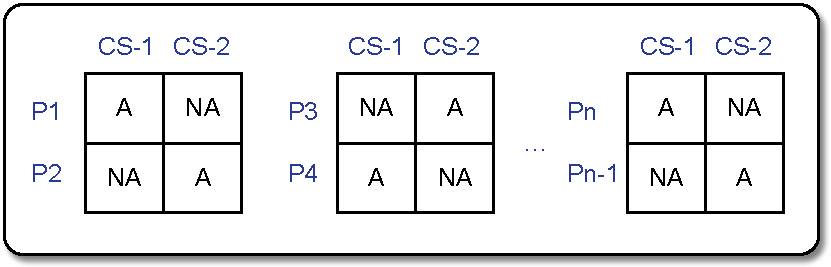
\includegraphics[scale=.50]{images/latin-square.pdf}
      \caption{Latin square design. Each ``square'' corresponds to 
      a replica in our study. Each replica comprises two participants (square rows, e.g., P1 and P2) 
      and two sets of programs (CS-1 and CS-2). We randomly apply the 
      treatments (atom or non-atom code) to the cells of the squares.} 
      \label{fig:latinsquare}
  \end{figure}

For each of the 10 selected atom candidates, we write one short program containing the atom. As in the repeated measures study, we call them the obfuscated versions of the programs. We also write corresponding short programs without the atom candidates and call them the clean versions of the programs. Overall, the experiment employed 20 programs, 10 obfuscated and 10 clean. In order to reduce the cognitive effort, each subject was asked to predict the output of 10 programs, five obfuscated and five clean. The order in which they are presented is randomized. By doing this, we seek to minimize the chances of subjects being aware that the current listing they are analyzing contains (or not) atoms of confusion. That is, each subject should indicate what would be the outcomes of the programs, some of them having atoms of confusion (while other programs do not). Since participants are not exposed to obfuscated and clean versions corresponding to the same atom candidate, learning effect is not possible. We measure answer correctness and the total time each participant requires to participate in the experiment.

{\bf Study instrument.} 
We implemented our experiment as a questionnaire in a web application and 
%carried out a pilot. 
%As part of this effort, we 
carried out an informal pilot. Undergraduate students and professional colleagues took part in the pilot. Some users reported layout defects, and many reported that the landing page did not explain the study well enough. We also spotted minor issues with our routines to create and populate the latin squares. 

We organize the questionnaire in three sections. The first section aims to characterize the subjects, asking their age, education level, and programming experience. We also include a check button, whose checking means users agree that all collected data will be used solely for research purposes. In the second section, we present to the participants a small set of instructions, where we explain how the study works and ask them to dedicate their attention to it. We stress to participants the importance of not using any aids during the experiment, such as online or console interpreters. For each question page, we kept track of whether or not the subjects switch windows. 

The last section of the questionnaire presents a sequence of ten questions, each containing a program. For each question, there is a text box where the answer should be written. There is also an ``I do not know'' button, which, when clicked, leads the subject to the next question. In our setting, ``I do not know'' is treated as a wrong answer. The programs are also presented as images copied from a text editor. Upon submitting their answer for a particular question, the subjects are automatically led to a similar page, containing another program. Similarly to the repeated measures study, we do not provide feedback about time and correctness to the subjects.


% \rb{nao acho esse paragrafo necessario} 
% \adriano{o de baixo ne? eu tambem acho}

% As we mentioned before, we first wrote the code listings in a text editor, and took pictures of it. In the case of an atom of confusion that was exclusive to JavaScript, which we called \textit{Automatic Semicolon Insertion} (see Appendix~\ref{sec:appendix-atoms}), it was necessary to remove the syntax highlighter. Even though semicolons at the end of statements are optional to programmers in JavaScript, the interpreter automatically inserts them into the code. Our text editor was incorrectly highlighting a line break after a return statement, even thought it was valid JavaScript syntax. We had thus to turn the highlighter off to take the picture of this atom. 

{\bf Study audience.}
We posted the invitation to take part in the study on a JavaScript Reddit channel.\footnote{https://www.reddit.com/r/javascript/} We explained our research purposes and asked developers of any level of expertise to take part. Within twelve hours, we collected more than 150 answers, populating more than 70 replicas of the Latin Squares. We collected significant data on time taken and discrepancies in answer correctness between obfuscated and clean versions of the programs. Some inconsistencies arose while building the squares, for instance, when a user quit in the middle of the questionnaire. We discarded from our study all squares that contained incomplete rows.

%Since we had a large enough number of samples, the squares we had to discard did not impact our analysis.

\subsection{Results}\label{sec:latin}

In the latin-square study, we estimate the impact of atoms considering the same two perspectives of the previous experiment: \emph{correctness} (number of wrong answers)
and \emph{time} (how long to provide a correct answer). In particular, in the time analysis, differently from the repeated  measures study, we compare the time required by participants to submit a correct response when analyzing code snippets with and without atom candidates. This study is based on the responses of 140 participants (a total of 70 replicas). All participants had taken at least some university course or hold a bachelor degree or equivalent. In addition, 21 participants hold a master's degree and three a doctorate degree. Considering the programming experience of our respondents, 19\% have more than ten years of programming experience, 37\% have between four and ten years of experience, 37\% have between one and four years of experience, and 7\% have less than one year of programming experience.  
Accordingly, we characterize the effect of atoms of confusion in JavaScript code taking into account the perceptions of both novice and experienced developers. 

\subsubsection{Correctness Analysis}
% \castor{We need to be uniform about terminology. Are we going with ``misunderstanding rate analysis''? The problem is that it is not clear to me to which rate this refers.}

{\bf Exploratory Data Analysis.}
As mentioned in Section~\ref{sec:meth:survey}, each participant in this experiment evaluated ten code snippets, from which five were in their obfuscated versions, whilst the other five contained clean versions of the code snippets (i.e., without the atom candidates). As in the repeated measures study, the participants should provide the expected outcomes of the code snippets. Differently from that study, in this one each participant only predicts the outcome of one version of each code snippet, either clean or obfuscated. As discussed, we collect information about \emph{correctness} (whether the participant correctly predicted the program's output) and \emph{time}. 
Table~\ref{tab:difference-correctness} and Figure~\ref{fig:boxplotcorrectness} summarize the results of the correctness experiment.

Considering Table~\ref{tab:difference-correctness}, the clean versions of six code snippets present at least a 15\% improvement in answer correctness when compared with the obfuscated versions. In particular, the presence of the \emph{Comma Operator} atom exhibits the highest impact on misunderstanding. 
Frequently used constructs and idioms, such as \emph{Post Increment} and \emph{Omitted Curly Braces} (see Section~\ref{sec:msr-results}), also result in many mistakes. %introduce high degrees of confusion.
The boxplot of Figure~\ref{fig:boxplotcorrectness} shows a non-negligible decrease in the average number of incorrect answers when observing the clean versions of the code snippets. Also, the sample of responses with no atoms had almost no dispersion, which supports the argument that the clean versions of the code snippets are easier to evaluate correctly. 


% \begin{table}[htbp]
% \caption{Difference in answer correctness between confusing and non-confusing pairs}
% \begin{center}
% \begin{small}
% \begin{tabularx}
% {{\linewidth}}{l p{1.5cm} p{1.1cm} p{1.1cm} p{1.2cm} }
% \textbf{Atom} & \textbf{\%Correct} & \textbf{\%Correct} \\
% &  \multicolumn{1}{l}{With AOC} \multicolumn{2}{l}{Without AOC}  & \Delta (\%)    \\
%  \hline
% Comma Operator & 40 & 93 & +132\%                 \\     
% Automatic Semicolon  Insertion & 46 & 97 & +110\% \\
% Post Increment & 69 & 91 & +31\%         \\
% Omitted Curly Braces & 67 & 83 & +23\%   \\ 
% Assignment as Value & 80 & 97 & +21\%    \\
% Implicit Predicate & 83 & 97 & +16\%     \\
% Logic as Control Flow & 59 & 68 & +15\%  \\
% Ternary Operator & 86 & 94 & +9\%        \\
% Pre-Increment & 71 & 76 & +7\%           \\
% Arithmetic as Logic & 91 & 90 & -1\%    \\
% \end{tabularx}
% \end{small}
% \end{center}
% \label{results_correctness}
% \end{table}

\begin{table}[htbp]
\caption{Summary of the correctness analysis}
\label{tab:difference-correctness}
\centering{
  {\scriptsize
  \begin{scriptsize}
\begin{tabular}{lrrr} \toprule
  Atom candidate& Obfuscated & Clean & $\Delta$(\%)  \\ \midrule
  Comma Operator                &  28 &  65 & +132   \\ 
  Automatic Semicolon Insertion &  32 &  68 & +112   \\ 
  Post-Increment                &  48 &  64 & +33    \\ 
  Omitted Curly Braces          &  47 &  58 &  +23   \\
  Assignment as Value           &  56 &  68 &  +21   \\ 
  Implicit Predicate            &  58 &  68 &  +17   \\ 
  Logic as Control Flow         &  41 &  48 &  +17   \\ 
  Conditional Operator              &  60 &  66 &  +10   \\ 
  Pre-Increment                 &  50 &  53 &  +6    \\ 
  Arithmetic as Logic           &  64 &  63 &  -2    \\ \bottomrule
  
\end{tabular}
\end{scriptsize}
}}
\end{table}

 %% Comma Operator          & 40 & 93  & +132 \\
 %% Post Increment          & 69 & 91  & + 31  \\
 %% Omitted Curly Braces    & 67 & 83  & +23 \\
 %% Assignment as Value     & 80 & 97  & +21 \\
 %% Implicit Predicate      & 83 & 97  & +16 \\
 %% Logic as Control Flow   & 59 & 68  & +15 \\
 %% Ternary Operator        & 86 & 94  & +9  \\
 %% Pre-Increment           & 71 & 76  & +7  \\
 %% Arithmetic as Logic     & 91 & 90  & +1  \\ \bottomrule


\begin{figure}[b!]
\noindent
 \centering
 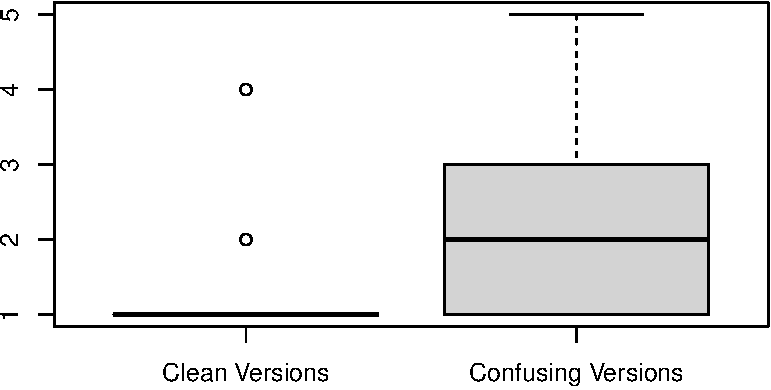
\includegraphics[width=0.6\columnwidth]{images/wrong-answers-plot-1.pdf}
 \caption{Number of wrong answers of each subject.}
 \label{fig:boxplotcorrectness}
 \end{figure}% \castor{Fiz de tudo para ajeitar a figura porque o texto embaixo deveria ser "Clean versions" e "Confusing versions" mas não sei porque não funcionou. Até mudei a figura. Não sei o que está havendo.}
 
% \rb{verificar a consistencia nas questoes de pesquisa mais especificas}

{\bf Statistical analysis.}
We first use the \emph{Pearson's Chi-squared test}
to investigate if there is a statistically significant difference in the frequency of correct and incorrect answers---due to the versions of the code snippets (obfuscated and clean code). The p-values for these tests are reported in the ``Chi-square test'' column of Table~\ref{tab:hypothesis-testing}. For five atom candidates (Comma Operator, Automatic Semicolon Insertion, Post-Increment, Assignment as Value, Implicit Predicate), the results indicate that the obfuscated versions of the code snippets have a negative impact on code understanding (p-value $< 0.05$). This result holds even after applying the Benjamini-Hochberg correction with a false discovery rate of 5\%. 

We measure the effect size of the clean version of the code snippets into the answers' correctness using the \emph{Odds Ratio} (OR). The results are reported in the ``Odds Ratio'' column of Table~\ref{tab:hypothesis-testing}. 
In the table, we also report the confidence interval (CI) for the OR in the ``CI'' column. Although many of the intervals are wide, for six of the atom candidates the lower bound of the confidence interval is greater than or equal to 1. This indicates that, at a 95\% confidence level, a developer is likely to commit less mistakes when using the clean versions. 
%Considering only the atoms for which there was a significant difference in correctness for confusing and clean versions and u
%Using the thresholds established by Chen and colleagues~\cite{Chen:2010:HBB} (OR = 1.68 small, 3.47 medium, and 6.71 large), 
For four of the atoms, Comma Operator, Automatic Semicolon Insertion, Assignment as Value, and Implicit Predicate, effect size can be considered large. For Implicit Predicate, it is medium. 
%We found a negligible effect size for the atom candidates Arithmetic as Logic, Logic as Control Flow, and Pre-Increment. Nonetheless, for the remaining candidates, the effect size is significant. 
For instance, when comparing clean and obfuscated code snippets pertaining to the Comma Operator atom candidate, we observed an \emph{Odds Ratio} of \num{19.02}. This means that the odds of a correct answer are \num{19.02} times higher when interpreting the clean version---in comparison with the corresponding obfuscated version of the code snippet. Furthermore, with a 95\% confidence level, the odds ratio is between 6.6 and 68.22, i.e., although the error margin is wide, it is strongly in favor of the clean version. If there is a significant likelihood of a developer committing a mistake when analyzing a clean version, the lower bound of the CI should be a number between 0 and 1 (since the OR is a ratio). This is the case for the four atom candidates in the lower part of the table. 
%In particular, in the last row (Arithmetic as Logic), the OR between 0 and 1 indicates that a participant was actually more likely to misunderstand the clean version. 

Finally, we also use a \emph{Binomial Generalized Logistic Regression} analysis to investigate if either \emph{participant education} or \emph{participant experience} impacts correctness. The findings suggest that \emph{participant experience} impacts the results related to correctness (p-value $<$ 0.001 and $\chi^2 = 24.18$).
Figure~\ref{fig:correctness-over-experience} summarizes the number of correct and incorrect answers over the four experience groups. Even though the presence of atoms of confusion reduces the number of correct answers for all \emph{experience groups}, this effect is not uniform. For instance, novice developers (under one year of experience) provide a higher number of wrong answers for the obfuscated version of the code (57.8\%), while developers with more than four years of experience provide more than 70\% of correct answers even when evaluating the obfuscated version of the code snippets. It is also important to note that, independently of the \emph{experience group}, developers tend to provide more than 84\% of correct answers while predicting the outputs for the clean versions of the code. We replicate the \emph{Pearson's Chi-squared test} for each experience group and find that the statistical difference is less significant for those developers with more than ten years of experience (p-value = 0.007 and $\chi^2$ = 7.08). Differently from \emph{participant experience}, the factor \emph{participant education} does not significantly change the correctness of the answers (p-value = 0.236 and $\chi^2$ = 5.54).

% \castor{I'd like to have the numbers for the results above. What are the p-values, regression coefficients, etc.?}

\begin{figure}
  \centering
  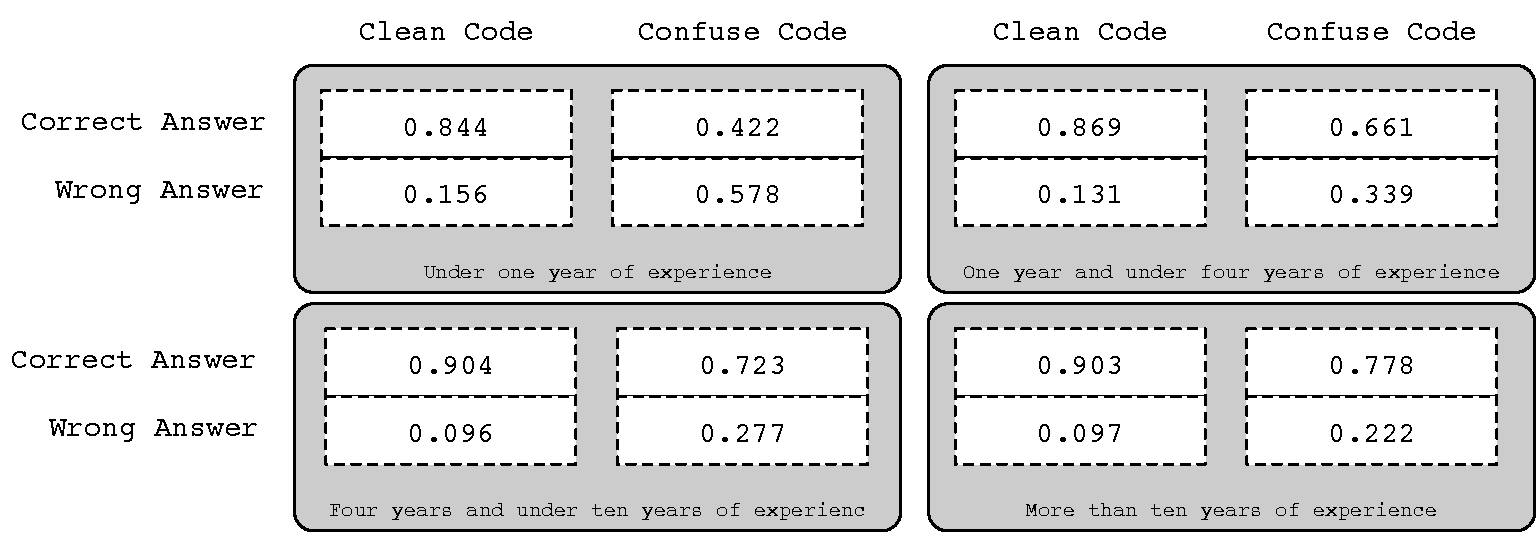
\includegraphics[scale=0.5]{images/correctness-by-experience}
  \caption{Impact of atoms of confusion on the correctness (over the four participant experience groups)}
  \label{fig:correctness-over-experience}
\end{figure}


%% \begin{mh}
%%   The results of our exploratory data analysis and   hypothesis testing suggest that the atom candidates Comma Operator, Automatic Semicolon Insertion, Post Increment, Omitted Curly Braces, Assignment as Value, and Implicit Predicate %, and Ternary Operator
%%   introduce some degree of misunderstanding in JavaScript code. %Based on the results of this study, 
%%   Therefore, they can be deemed atoms of confusion for JavaScript.
%% \end{mh}

%% \begin{mh}
%% {\color{red}Comparing the results of different studies,
%%   the impact of atoms candidates on source code
%%   (mis)understanding differ according to the programming
%%   language.}
%% \end{mh}
%% Regarding the first question we 
%% address in the survey (\emph{Do code snippets that contain atoms of confusion produce a higher error rate than snippets where the atom is removed?}), we found evidence that the atoms of confusion lead programmers to misunderstand JavaScript code. We also realized that just one atom whose correction has a non-significant improvement in the percentage of correct answers---we found an improvement of at least 15\% in the correct answers when removing the confusing code for seven atoms (out of ten atoms we consider in the survey). 

\subsubsection{Time Analysis}

{\bf Exploratory Data Analysis.}
Table \ref{tab:difference-time-taken} shows the average time necessary for the participants to give a correct answer about the expected outcomes of a code snippet, considering both obfuscated and clean versions. We do not consider cases where the participants made mistakes. Seven atom candidates required more time from participants to predict a correct response. For these eight atom candidates, developers take at least 5.90\% less time on average to find a correct answer when considering the clean version of a code snippet. In the extreme case (atom candidate Comma Operator), the participants take 76.23\% less
time on average to find the correct answer for the clean version of the code snippets. 
Not all atom candidates, though, require less time for the participants to predict the answer. In fact, for  Arithmetic as Logic and Pre-Increment, the time to give a correct answer for the clean versions was   
29.06\% and 38.19\% smaller than for the obfuscated versions---we did not confirm these atom candidates as atoms of confusion in the previous section.

\begin{table}[htbp]
\caption{Time in seconds to submit a correct answer}
\centering{
  {\scriptsize
  \begin{scriptsize}
\begin{tabular}{lrrr} \toprule
Atom & Obfuscated  & Clean & $\Delta$(\%) \\ \midrule
Comma Operator & 87.67 & 20.84 & -76.23 \\ 
Automatic Semicolon Insertion & 46.08 & 22.04 & -52.17 \\ 
Post-Increment & 28.70 & 25.67 & -10.56 \\ 
Omitted Curly Braces & 48.85 & 30.00 & -38.58 \\ 
Assignment as Value & 52.47 & 48.95 & -6.71 \\ 
Implicit Predicate & 36.24 & 24.01 & -33.75 \\ 
Logic as Control Flow & 108.94 & 51.07 & -53.12 \\ 
Conditional Operator & 41.80 & 39.34 & -5.90 \\ 
Pre-Increment & 30.71 & 42.45 & 38.19 \\  
Arithmetic as Logic & 28.82 & 37.20 & 29.06 \\ \bottomrule
\end{tabular}
\label{tab:difference-time-taken}
\end{scriptsize}
}}
\end{table}

 % latex table generated in R 4.0.4 by xtable 1.8-4 package
 % Thu Apr 22 07:58:21 2021
 \begin{table*}[ht]
\caption{Hypotheses Testing (misunderstanding and time). Asterisks ($^{*}$) indicate a statistically significant difference.}
 \centering
 {\scriptsize
 \begin{tabular}{lrrr|rr}
   \toprule
      & \multicolumn{3}{c}{Correctness analysis} & \multicolumn{2}{c}{Time analysis} \\ \toprule
Atom  & Chi-square & Odds           & Confidence & Mann-Whitey& Cliff's\\ 
 &  test &Ratio          & Interval &  U test & Delta \\  \midrule
Comma Operator & \textbf{$<$ 0.0001*} & 19.02 & (6.60, 68.22) & \textbf{$<$ 0.0001*} & -0.53 \\ 
Automatic Semicolon Insertion & \textbf{$<$ 0.0001*} & 39.33 & (9.21, 356.62) & 0.0980 & -0.16 \\ 
Post-Increment & \textbf{0.0015*} & 4.83 & (1.73, 15.74) & 0.1201 & 0.15 \\ 
Omitted Curly Braces & 0.0510 & 2.35 & (1.00, 5.77) & 0.9253 & -0.01 \\ 
Assignment as Value & \textbf{0.0035*} & 8.39 & (1.81, 79.12) & 0.8268 & 0.02 \\ 
Implicit Predicate & \textbf{0.0112*} & 6.95 & (1.46, 66.56) & \textbf{0.0029*} & -0.29 \\ 
Logic as Control Flow & 0.2920 & 1.54 & (0.73, 3.28) & \textbf{$<$ 0.0001*} & -0.39 \\ 
Conditional Operator & 0.1590 & 2.73 & (0.74, 12.57) & 0.2407 & -0.12 \\ 
Pre-Increment & 0.7015 & 1.25 & (0.55, 2.85) & \textbf{0.0062*} & 0.27 \\ 
Arithmetic as Logic & 1 & 0.84 & (0.22, 3.12) & \textbf{0.0172*} & 0.23 \\ 
    \bottomrule
 \end{tabular}}
 \label{tab:hypothesis-testing}
 \end{table*}


{\bf Statistical analysis}
We use the \emph{Mann-Whitney U test} to
investigate the null hypothesis that developers 
spend the same amount of time to correctly
predict the outcome of clean and obfuscated versions of a code snippet.
%, regardless of evaluating the confusing or clean version of the code.
The results of Table~\ref{tab:hypothesis-testing}
suggest that we should refute the null hypotheses for five atom candidates (Comma Operator, Implicit Predicate, Logic as Control Flow, Pre-Increment, and Arithmetic as Logic), after applying the Benjamini-Hochberg correction with a false discovery rate of 5\%. For the first three, the analysis suggests that the participants need more time to predict the outcome of the code snippet in the obfuscated code version. For the atom candidates Arithmetic as Logic and Pre-Increment, the participants take less time to predict the outcome of the code snippets in the obfuscated version. We also computed the effect size using Cliff's Delta statistic. In the table, negative effect sizes suggest that it took less time to correctly predict the output of clean versions of the snippets.  Considering the thresholds established by Romano et al.~\cite{Romano:2006:ASO} (0.147 $<$ $|$d$|$ $<$ 0.33 small, $|$d$|$ $<$ 0.474 medium, otherwise large), we found a large effect for the Comma Operator atom candidate; a medium effect size for Logic as Control Flow, and small effect sizes for Automatic Semicolon Insertion, Implicit Predicate, Arithmetic as Logic, Post-, and Pre-Increment. 


%% \begin{mh}
%%   The results suggest that developers tend to spend
%%   more time to predict the correct answer in the presence of the atom candidates Comma Operator, Logic as Control Flow, and Implicit Predicate. Conversely, the code snippets with the atom candidates Arithmetic as Logic and Pre-Increment demand less time to predict the correct answers. 
%% \end{mh}


%%  Comma Operator        & 60 & 21  & -65  \\
%% Logic as Control Flow & 85 & 49  & -42  \\
%% Implicit Predicate    & 33 & 24  & -27  \\
%% Omitted Curly Braces  & 43 & 31  & -27  \\
%% Assignment as Value   & 53 & 49  & -7   \\
%% Ternary Operator      & 42 & 42  & 0    \\
%% Post Increment        & 27 & 27  & 0    \\
%% Arithmetic as Logic   & 29 & 36  & +24  \\
%% Pre-Increment         & 34 & 49  & +44  \\


% \rb{acho que podemos melhorar a apresenta\c c\~{a}o dessas tabelas, talvez usando booktabs.}



\section{Interview Study}\label{sec:method:interview}

To complement the two experiments, we perform semi-structured interviews with professional JavaScript developers, aiming to identify their perceptions regarding programs containing atoms of confusion (research question RQ2). We also ask each participant if they know of any other JavaScript-specific construct or idiom they think is likely to make the code hard to understand. % (research question RQ3). 
In this section we detail the protocol we followed to conduct the interviews and to analyze the results.

% Nós realizamos entrevistas semi-estruturas com o objetivo de identificar a percepção dos desenvolvedores com experiência em JavaScript sobre algumas questões relacionadas à compreensão de código em JavaScript. Assim, nesta Seção nós descrevemos os procedimentos adotados para selecionar os participantes para as entrevistas e detalhamos como as entrevistas foram conduzidas. Além disso, detalhamos como os resultados das entrevistas foram analisados.

\subsection{Participant Selection} We invite the participants of the interviews using a snowballing technique. That is, starting from our network of contacts, we invite an initial set of candidates to take part in our experiments. From this initial list, we ask for an indication of additional candidates. Our main selection criterion is that all participants should have been working with JavaScript in their daily professional activities. We invited a total of 17 developers, and 15 of them agreed to participate.   
%We conducted the interviews for a period of two weeks.


\subsection{Interview Process} We conduct semi-structured interviews using web conferencing software. We record all the interviews with the consent of the participants. On average, the interviews last 26.29 minutes, with the shortest one lasting 14.59 minutes and the longest one 43.06 minutes. Two of the researchers conduct the interviews, and a third one listens to all the recordings to cross-validate the collected data. The interviews have three main parts. In the first one, we ask the developers the following demographic information: name, email, gender, level of education, current job position, JavaScript experience in years, and other programming languages they have worked with. Table \ref{pinterview} summarizes this demographic information.

\begin{table}[htb!]
  
  \centering
  \caption{Demographic information of the participants}
\begin{scriptsize}  
\begin{tabular}{clcl}
\toprule
ID & Education & JS Experience & Other Languages \\ \midrule 
P1 & BSc Degree & 9 years & Java, PHP, C, Go  
\\ 
P2 & HS Degree & 3 years & Python, Go, Dart, Lua, C++, C\#
\\ 
P3 & BSc Degree & 4 years & Java, C
\\ 
P4 & Undergraduate & 3 years & Python, C, C++, Java, Go
\\ 
P5 & Master Student & 3 years & Python, SQL
\\ 
P6 & Bsc Degree & 15  years  & Java, PHP, C, Python , Ruby, C\#
\\ 
P7 & BSc Degree  & 6 years & C, C++, Java, Assembly, Kotlin
\\ 
P8 & PhD Degree & 2 years & Java, Python
\\ 
P9 & BSc Degree  & 5 years & PHP
\\ 
P10 & Master Student & 4 years & Java, C\# and Python
\\ 
P11 & Master Student & 4 years & Java, Erlang, C\#, Cobol
\\ 
P12 & Master Degree & 1 year & C
\\ 
P13 & Master Degree & 13 years & Java, PHP
\\ 
P14 & Master Student & 3 years & C, Python, Ruby
\\ 
P15 &  BSc degree  & 2 years & Java, PHP
\\ \bottomrule
\end{tabular}
\end{scriptsize}
    \label{pinterview}
\end{table}

In the second part of the interview our aim is to allow the subjects to describe their JavaScript experience, as well as to allow them to reveal any JavaScript constructs they regard as innately confusing. This allows us to identify potential atom candidates that are more specific to the JavaScript language. Examples of questions we explore in this section include: \emph{Does JavaScript favor developers to produce code that is hard to understand?} and \emph{Do you regard any particular construct or idiom of the language as especially confusing?}

In the third part of the interview, participants are shown pairs of programs that were used in the experiments, where each pair contains a clean and an obfuscated version of the same atom candidate. For this part we only use atoms that appear in both experiments. The participants 
are asked to evaluate which version of the code is easier to understand. To avoid introducing bias in the answers, the interviewers do not explain that one of the versions in each pair contains the atom under investigation. Subjects are just presented the pairs of programs and allowed to take the necessary time to decide on the most readable one.

\subsection{Interview Analysis}

We first transcribe each interview and then examine the broad distribution of the answers. Our goal is to build an initial understanding of the participants' perceptions with regards to the challenges to understand JavaScript code in general and JavaScript code with atoms of confusion in particular. We follow-up with an open-coding procedure, highlighting the main themes and quoting the answers of the participants. We present these results in Section~\ref{sec:interview-results}. 


\subsection{Results}\label{sec:interview-results}

In this section we present the results of the interviews with the practitioners. We contrast the findings of the experiments of Sections~\ref{sec:repeated} and~\ref{sec:latin} with the opinion of software developers about their preferences regarding the obfuscated or clean versions of the code snippets. For the interview study, we only considered atoms that were analyzed in both the repeated measures (Section~\ref{sec:repeated}) and the latin square (Section~\ref{sec:latin}) studies. 

A total of 15 practitioners took part of the interviews.
We collected information regarding programming
experience, familiarity with JavaScript, and their opinion about the \na atom candidates we explored in the both experiments. We first presented them pairs of clean and obfuscated code snippets and then asked them to discuss their preferences towards one version. We did not indicate in any way whether any version was assumed to be confusing or not. 

\begin{table}[!htb]
    \centering
    {\scriptsize
    \caption{Summary of participants' preferences for code snippets \emph{with} and
      \emph{without} atom candidates. The participants were only presented the code snippets, without any indication about whether one was confusing or not. 
      Participants were also allowed to choose Neutral when they thought both sides were equally readable.}\label{tab:interview-results1}
    \begin{tabular}{lrrr}\toprule
      & \multicolumn{3}{c}{\textsc{Preference (\%)}} \\
      \cmidrule(lr){2-4}
         Atom           & \multicolumn{1}{c}{Obfuscated}
                                      &  \multicolumn{1}{c}{Clean}
                                               & \multicolumn{1}{c}{Neutral} \\ \midrule
         Comma Operator                  & 0  & 100    & 0     \\
         Automatic Semicolon Insertion  & 0  & 80     & 0     \\
         Post-Increment                  & 20 & 73.33  & 6.67  \\
         Omitted Curly Braces            & 0  & 100    & 0     \\
         Assignment as Value             & 20 & 60     & 20    \\
         Implicit Predicate              & 20 & 73.33  & 6.67  \\
         Logic as Control Flow           & 20 & 60     & 20    \\
         Conditional Operator                & 60 & 26.67  & 13.3  \\
         Pre-Increment                   & 40 & 46.67  & 13.33 \\ 
         Arithmetic as Logic             & 0  & 93.33  & 6.67  \\ \midrule
         \textsc{overall}                & 18 & 71.33  & 8.64  \\
         \bottomrule
    \end{tabular}
    }

\end{table}

\subsubsection{The Participants' perceptions of the atom candidates} 

Supporting the results of Sections~\ref{sec:repeated} and~\ref{sec:latin}, Table~\ref{tab:interview-results1}
 shows that for eight out of the
10 scenarios surveyed, the majority of the respondents prefer the version of the
code without the atom candidate.
In no case the \emph{neutral}
ratio was higher than the option for the clean version.
%% An example entry is contained in Appendix~\ref{}. 
%% For a full listing of the code snippets, visit the paper repository. 
Only for the Conditional Operator atom candidate the participants preferred the obfuscated version, instead of the clean one. Figure~\ref{code:ternary} shows the code snippets for the corresponding obfuscated and clean versions. For this atom candidate, some participants who preferred the left-hand side version (obfuscated) still believed that the right-hand side version (clean) was more readable. The following quotes were extracted from the transcripts with
% three interviewees:
two interviewees:

\begin{figure*}

\noindent\begin{minipage}{.45\textwidth}
\begin{lstlisting}[language=JavaScript, caption=\emph{Left-hand side} (using the \emph{Conditional Operator} atom).]
let config = {size: 3, isActive: false};
const_config = config.isActive === true 
             ? config 
             : {size: 10};
console.log(_config.size);
\end{lstlisting}
\end{minipage}\hfill
\begin{minipage}{.45\textwidth}
\begin{lstlisting}[language=JavaScript, caption=\emph{Right-hand side} (without the atom).]
let config = {size: 3, isActive: false}
let _config;
if(config.isActive === true) {
  _config = config;
}
else{
   _config = {size: 10};
}
console.log(_config.size);
\end{lstlisting}
\end{minipage}
\caption{Example of a pair of code snippets used in the interview pertaining to the \emph{Conditional Operator} atom candidate}
\label{code:ternary}
\vspace{-0.2cm}
\end{figure*}

\begin{mq}
\emph{``I prefer to write [code using the \lhs version], but I think [the \rhs version] is easier to read, especially for newer programmers''}.
\end{mq}

\begin{mq}
\emph{``When I am programming, I write code with the conditional operator, [...], but, to be honest, I still think that 
[the code using the \rhs version] 
is easier to understand''}.
\end{mq}

%% \begin{mq}
%% \emph{``I think [the \lhs version] is easier to understand, but [the \rhs version] is what I would write"}
%% \end{mq}

%% The atom candidate Ternary Operator also opens up
%% the possibility for a derivative construct that JavaScript
%% allows which can be rather confusing, and that is the nested
%% ternaries construct, in which the right-hand side of the a
%% ternary operator can be another ternary construct.
%% While nested ternaries remove the number of lines that
%% would be necessary to construct using nested if-then-else statements,
%% they can become quite taxing to understand.
%% Nested ternaries are a choice of atoms to be analyzed in future work.

The Pre-Increment atom candidate also caused a
conflict in one of the interviewees, who
regarded the clean version as simpler to understand, but would still opt to write
code with the atom. In contrast, %to such opinion,
one of the participants found the version with the atom candidate more elegant, but recognized it was less readable, and was willing to sacrifice elegance for readability. In the repeated measures study, we found a significant difference in favor of the clean version, with a large effect size in its favor. In the latin square study, no difference could be observed in terms of correctness. However, there was a significant difference in terms of the time required to predict the output correctly in favor of the obfuscated version. 
%% \rb{pela discuss\~{a}o anterior, parece-me que alguns
%%   desenvolvedores reconhecem que esses candidatos
%%   a \'{a}tomos introduzem certa dificuldade de compreens\~{a}o;
%%   mas mesmo assim optam por usar a constru\c c\~{a}o correspondente.
%%   Acho que cabe um box aqui com essa discuss\~{a}o sobre isso.}

When analyzing the Logic as Control Flow atom candidate, one of the interviewees gave an example of personal experience that might motivate one to avoid writing code using this construct:

\begin{mq}
  \emph{``This one is interesting, because I have written code that looks like the left-hand side [obfuscated version], and my colleagues complained that it was difficult to understand. Nowadays I prefer to write code using the version on the right-hand side [clean version]''}.
\end{mq}
\noindent
None of the two studies found a significant difference in correctness between clean and obfuscated versions of snippets related to this atom candidate. However, in the latin square study the participants analyzing clean versions of the snippets required significantly less time. 

For two of the atom candidates, the interviewees were unanimous in their preference for the clean version: Comma Operator and Omitted Curly Braces. Not coincidentally, in both experiments there were significant differences in correctness in favor of the clean versions for both atoms. Regarding the first one, we could often notice during the interviews that the \emph{\lhs} (with the atom of confusion) caused significant confusion among the participants. One remark about the \emph{Comma Operator} atom of confusion is listed below:

%% \begin{mq}
%% \emph{``I just learned that [the \lhs version of this code] is possible. I did not even know it worked''}
%% \end{mq}

\begin{mq}
\emph{``The code in [the \lhs version] is unlikely to be understood unless the programmer knows \clang or \cpplang''}.
\end{mq}

As for the atom candidate Omitted Curly Braces, one of the interviewees mentioned that, although they understand why one would opt not to use braces for simple if-then-else statements, they still advised against it, on grounds that:

\begin{mq}
\emph{``[I prefer the \rhs version of the code \ldots]
If I want to see well-written, easily understandable code, then I also have to do my job. Therefore I believe that, since I do not know who is on the other end maintaining this code, and it could be any person with any level of expertise, then I try to write readable, easy-to-understand code''}.
\end{mq}

%This is an interesting perspective, because such a perhaps simple decision,  might hinder novice developers in the task of maintaining code; and one cannot make any assumption about the programmers' experience of who is going to maintain a code in a long run.

%This is an interesting perspective because such a simple decision might hinder novice developers in maintaining code; one cannot assume the programmers' experience of who will maintain a code in the long run.



\subsubsection{Confusion in JavaScript Code} 

% The final remarks that were drawn from the interviews are related to potentially confusing constructs that were suggested by the participants, as well as their perspective on JavaScript as a language, from which we can also uncover some other forms in which the language itself might contribute to writing confusing code.

The final remarks drawn from the interviews are related to potentially confusing constructs suggested by the participants and their perspectives on JavaScript as a language. From the latter, we can also uncover some other forms in which the language itself might contribute to writing confusing code.

One of the participants mentioned that the use of JavaScript's prototype-based inheritance can make it difficult to understand code, particularly when involving deep prototype chains.
%This is a core feature of the language, and most high-level tools and frameworks abstract it away.
%Although this was only mentioned by one practitioner, this is an important remark, as true understanding of JavaScript software necessarily involves understanding the concept of prototypes.
% When asked about particular JavaScript constructs or patterns that can make code difficult to understand, three participants cited the callback pattern, which can lead to several levels of nested function calls, as extremely difficult to assimilate.
When asked about particular JavaScript constructs or patterns that can make code difficult to understand, three participants cited the callback pattern---potentially leading to several levels of nested function calls---as extremely difficult to assimilate. One of the respondents stated:

\begin{mq}
\emph{``Nested callbacks are very confusing. Even writing them can be confusing, let alone understanding them.''}
\end{mq}

Two other developers implicitly touched upon the callback pattern, mentioning that it can be difficult to understand \emph{asynchronous} programming in JavaScript.
%Since what is really happening at a lower level is that the JavaScript engine creates a callback stack that is separate from the main execution stack, and that callback functions are only executed when the main execution stack is empty, the concepts of asynchronous events and callbacks are inseparable in the language, and any abstractions for callback functions, such as promises and async/await syntax only hide the pattern.
We also found other idioms that are JavaScript atom candidates, including
\emph{property access} via array subscription (\lstinline[language=javascript]{V1['P1']} instead of \lstinline[language=javascript]{V1.P1}) and \emph{arrow functions} (see listings~\ref{arr1} and~\ref{arr2}). The former was investigated in the repeated measures study but we did not find a significant difference between clean and obfuscated versions. As future work, we aim at investigating whether or not these atom candidates are more likely to introduce confusion in JavaScript code.

\begin{figure}
\begin{small}
\begin{lstlisting}[language=JavaScript,caption=Example of arrow function.,label=arr1]
let inc = (x) => x + 1;
\end{lstlisting}
\begin{lstlisting}[language=JavaScript,caption=Alternative version without arrow function.,label=arr2]
let inc = function(x) {
  return x + 1
}
\end{lstlisting}
\vspace*{-0.6cm}
\end{small}
\end{figure}

\section{Discussion}
\label{sec:discussion}

\castor{Which atoms? The weight of experience. Statistical significance vs. practical relevance. Most of them, with the exception of Comma Operator and Object Destructuring, have also been observed for Java programs~\cite{Langhout:2021:ACJ}.

In addition, many of the coding idioms that have been previously identified as atoms of confusion in previous work~\cite{DBLP:conf/sigsoft/GopsteinIYDZYC17,Langhout:2021:ACJ}, such as Logic as Control Flow

Differences among the two studies, for example, post increment was not significant in the first one but it was significant in the second.
}

Our work has several implications.
First, it adds external validity to the
work of Gopstein et al.~\cite{DBLP:conf/sigsoft/GopsteinIYDZYC17},
which investigates
the impact of atom candidates on
understanding \clang,\cpplang code. That is,
similarly to their work, the atom candidates
Comma Operator, Post/Pre Increment, Omitted Curly Braces,
Assignment as Value, Implicit Predicate, and Logic as
Control Flow seem to make 
JavaScript code harder to understand. For five of them, the difference is statistically significant, with a large effect size for four atoms. Our results also 
refute the hypothesis that Arithmetic as Logic is an atom of confusion (i.e., a source of misunderstanding).
In comparison to the original
work of Gopstein et al.~\cite{DBLP:conf/sigsoft/GopsteinIYDZYC17}, 
our study
led to some differences in the effect size
of the atom candidates.
Altogether, we answer our first research question.

\begin{mh}
  {\bf Answer to RQ1:} The first study (survey) gives evidence that some of the atom candidates in \clang and \cpplang programs that also exist in JavaScript correspond to a source of misunderstanding in
  JavaScript code. 
\end{mh}

The results of the interview study complement the understanding of atoms of confusion because the participants make clear the existence of a trade-off between code comprehension and other quality attributes. For instance, most of the participants prefer the version of the code with the Conditional Operator, even though they agree that its use might contribute to the misunderstanding of JavaScript code, particularly when novices are maintaining the codebase. The participants of the interview study also
mentioned other possible sources of misunderstanding in JavaScript,
including the use of prototype-based inheritance and nested call-backs (as discussed in Section~\ref{sec:interview-results}). Other JavaScript atom candidates include
Object Destructuring, Array Spread, Object Spread, and Type Conversion.
In summary, the results of the second study (interviews) allow
us to answer the second research question.

\begin{mh}
  {\bf Answer to RQ2:} The qualitative analysis of the
  interviews supports the results of the first study,
  since JavaScript developers most often agree that atoms of confusion compromise
  source code understanding. 
\end{mh}

%% \begin{mh}
%%   {\bf Answer to RQ3:} The qualitative analysis of the
%%   interviews suggests that specific JavaScript constructs might also correspond to atoms of
%%   confusion, including prototype inheritance and
%%   nested callbacks. 
%% \end{mh}

The results of the third study (mining open source
JavaScript repositories) provides evidence that,
although atoms of confusion compromise program
comprehension, they frequently appear in open
source JavaScript projects. In particular,
seven, out of 10 atoms considered
  in our study, appear in more than 50\% of
the 72 projects we analyzed. Furthermore, at least two of them are used intensively, more than once for every 200 lines of code. In summary, the third study
allows us to answer the third research
question.


\begin{mh}
  {\bf Answer to RQ3:} The MSR study reveals that
  the several atom candidates explored in our research
  appear frequently in practice, and cleaning up the use of 
  Post-Increment/Decrement and the Automatic Semicolon Insertion
  might improve the readabiliy of JavaScript code substantially. 
\end{mh}



%% We conducted a non-exact replication of the three
%% studies (survey, interview, and mining software repositories)
%% considering these more specific JavaScript atom candidates.
%% We confirmed that they truly correspond to sources of misunderstanding.
%% Due to lack of space,
%% we cannot present all the results here, and we postpone the presentation of these results as future work.




\section{Threats to Validity}
\label{threat}

In this section we discuss some of the main threats to the validity of this work. 

%Conclusion validity is connected with how well it is possible to establish relationships between treatments and outcomes. Threats to conclusion validity often come from inappropriate use of statistics. 

\textbf{Conclusion validity.} 
%Threats to conclusion validity often come from inappropriate use of statistics. 
In the context of our survey study, we apply different non-parametric statistical tests appropriate for the cases where data was categorical (correctness, Chi-square test of independence) and continuous (time, Mann-Whitney U test). Furthermore, besides reporting p-values, we also report effect size measures appropriate for each scenario (odds-ratio and Cliff's delta) and apply a p-value correction technique to avoid the multiple testing problem. Finally, it could be argued that the size of the samples is insufficient to make conclusions for some of the atoms, a common problem in Empirical Software Engineering. We estimate the sample size for each one of the atom candidates, considering that each one had a different number of samples (Table~\ref{tab:difference-correctness}). To that end, we use the $\phi$ measure of effect size for each atom (based on the Chi-square statistic), the standard $\alpha$ coefficient of 0.05, and set the expected statistical power to 0.8, as usually employed in the literature~\cite{Ellis:2010:EGE}. We find out that the sample size is sufficient for all but one of the atoms where we had a statistically significant result for correctness, Implicit Predicate. 
% For the ones where we did not find statistically significant results for correctness, in fact the sample sizes
% we have analyzed are insufficient for such small effect sizes. This indicates that further studies on these
% atoms are required, due to the likelihood of type II errors.

%Construct validity is connected with how well the selected measures actually represent the concept of interest. 

\textbf{Construct validity.} We use correctness as a proxy for program comprehension and predicted outcomes of small programs as a measure of correctness. As discussed elsewhere~\cite{Oliveira:2020:ECR}, this approach is a test of the developers' ability to trace programs. Although this is a common approach in studies about atoms of confusion~\cite{TheEyesDoNotLie,Langhout:2021:ACJ,DBLP:conf/sigsoft/GopsteinIYDZYC17}, other measures of correctness could have been employed, potentially yielding different results. As a complement to correctness in the survey, we have measured the time it took for the participants to correctly predict the outcome of the code snippets (either with or without atom candidates). Furthermore, we have  asked the interviewees about their preferences when comparing confusing and clean versions of the programs.

%A potential problem with our method is that there little incentive for subjects to think thoroughly about the questions. We observed a lack of engagement when we ran the survey with undergraduate students during a pilot study. Although our final subjects were voluntarily partaking in the survey, we could not be sure that, after some time taking the survey, respondents would become tired and stop thinking clearly about the code.


%Internal validity is concerned with how well the study isolates the variables of interest and accounts for confounding factors. 

\textbf{Internal validity.} Since the survey was conducted online with unknown participants, we have no way of confirming their levels of education and experience. We mitigate this threat by, in the data analysis, explicitly accounting for programmer experience and using an experimental design that allows us to isolate the impact of the treatment from factors such as experience and formal education level. Also, we did not have a way to prevent respondents from cheating, such as running the code on an interpreter, or consulting other people. We partially mitigate this threat by presenting images with source code, instead of text. This creates an obstacle for participants to run the code while taking the survey.

%External validity is linked to whether it is possible to extrapolate the results of the study. 

\textbf{External validity.} Our results suggest that the selected idioms and code constructs may lead to confusion for small code snippets, but it is not clear if that result extrapolates to other scenarios. Even though it is likely that in larger code bases the confusion induced by these constructs may be even greater, the existence of additional context may mitigate this effect. Another possible threat to the generalizability of our results, in particular for the survey and interviews, lies in the fact that the analyzed atoms may rarely occur in real JavaScript code bases. To mitigate that threat, we have analyzed 72 popular open source JavaScript repositories and found out that most of them are common, occurring at least once per 1,000 lines of code. Only Arithmetic as Logic and Comma Operator occur less frequently than once per 10,000 lines of code.

\revised{\textbf{Precision of our CodeQL queries.}
  We relied on existing CodeQL JavaScript predicates to implement most of our source code queries. However,
  we still had to implement our own predicates for three specific queries: the queries that search for the atoms Automatic Semicolon Insertion, Comma Operator, and Omitted Curly Braces.
  Figure~\ref{lst:codeql-automatic} shows examples of predicates we have implemented. Our test cases and manual assessments revealed that our queries correctly identified the
  atoms in the source code. Unfortunately, we observed that a predefined CodeQL predicate (named mayHaveBooleanValue) we used to mine the Implicit Predicate atom might have
  produced many false positives. That is, there are situations where this predicate wrongly states that an expression does not have a boolean value.
  This issue might have inflated the number of Implicit Predicate occurrences we reported in Section~\ref{sec:s04}}.

\begin{figure}[htb]
\begin{lstlisting}[language=CodeQL, basicstyle=\scriptsize]
import javascript

predicate hasTokenAfter(ReturnStmt r) {
  r.getLastToken().getNextToken().getValue() != "}"
}


predicate isNextTokenVariable(ReturnStmt r) {
  r.getLastToken().getNextToken() instanceof IdentifierToken and 
  r.getLastToken().getNextToken().getNextToken().getValue() != "="
}


predicate isNextTokenLiteral(ReturnStmt r) {
  ( r.getLastToken().getNextToken() instanceof StringLiteralToken or
    r.getLastToken().getNextToken() instanceof NumericLiteralToken ) and 
  r.getLastToken().getNextToken().getNextToken().getValue() != "="
 }

from ReturnStmt r
where not r.getTopLevel().isMinified() and
 r.isSubjectToSemicolonInsertion() and 
 r.getNumChildStmt() = 0 and
 r.getNumChildExpr() = 0 and
 not r.toString().matches("%;") and
 hasTokenAfter(r) 
select r, r.getLocation().getStartLine(), r.getLocation().getFile()
\end{lstlisting}
  \caption{CodeQL query that searches for the atom Automatic Semicolon Insertion. Note that, for this query,
    we had to implement three CodeQL predicates.}
  \label{lst:codeql-automatic}
\end{figure}
% \castor{A forma como os átomos foram detectados é uma ameaça que não discutimos.}


%% Finally, in one of the atoms, namely the Omitted Curly Braces,
%% we intentionally removed indentation from the original code,
%% which is highly unusual, given that many programmers use automatic
%% formatting in their code editors. This can introduce some level
%% of artificiality to this atom's question. Nonetheless,
%% we discovered that JavaScript does allow the programmer
%% to omit the curly braces after \textit{if} statements,
%% and insert multiple statements in the following line.
%% This fact itself might constitute
%% a source of confusion, which we leave to analyse
%% in our future endeavors. 

\section{Conclusions}
\label{conclusion}

This paper reports the results of a mixed-method research effort that allowed us to better understand the impact of atoms of confusion in JavaScript code. This involved a repository mining study, two experiments, and an interview study. The two independently-conducted experiments, which involved 210 JavaScript developers in total, asked them to predict the output of code snippets with and without atoms candidates. In at least one of the experiments, five atom candidates (Type Conversion, Change of Literal Encoding, Omitted Curly Braces, Pre-Increment, and Post- Increment) significantly impact program comprehension activities and can be considered atoms of confusion.
%% : Comma Operator, Automatic Semicolon Insertion, Post Increment, Assignment as Value, and Implicit Predicate. 
%% We also interviewed 15 professional developers. In general, they considered code without atom candidates easier to understand and highlighted other JavaScript constructs and idioms that might also introduce misunderstanding. 
%Last, but not least,
%Finally, we conducted a mining software repositories study. We found four atom candidates frequently used in JavaScript code, i.e., Implicit Predicate, Post Increment, Ternary Operator, and Omitted Curly Braces.  %The first two can be considered atoms of confusion. 
Our efforts have two implications for practice. First, we present evidence that not all atoms of confusion validated to \clang, \cpplang, or Java led to a statistically significant impact on program understanding for JavaScript. Besides that, our findings might be used to alert developers to avoid writing JavaScript code with certain atoms of confusion (e.g., Comma Operator, Automatic Semicolon Insertion, Post Increment/Decrement, Assignment as Value, and Implicit Predicate). Finally, our results might help tool developers to create program transformation tools for removing atoms that frequently appear in software. 
%They might firstly focus, for instance, on the atoms we found to be more confusing and at the same time more common in practice (e.g., Omitted Curly Braces and Post Increment).
%Promising candidates may be the atoms we found to be most confusing and, at the same time, common in practice (e.g., Implicit Predicate and Post Increment).
%As mentioned, the results of the interviews
Our research also pointed out additional JavaScript constructs and idioms 
that might introduce misunderstanding. These include nested callbacks, % and prototype-based inheritance (which might not have a counterpart version), but also idioms such
%as 
\emph{property access}, and \emph{arrow functions}. As future work, we intend to
reproduce our survey to validate whether or not these additional
idioms 
%, which the interviewees pointed out, 
truly affect
the understanding of JavaScript code. 



% \section*{Acknowledgment}
{\small
\bibliographystyle{elsarticle-num-names} 
\bibliography{reference}
}
\end{document}
